\documentclass[a4paper, 12pt, openany]{book} %chose the paper size and font size. Openany ensures that all all chapters and similar may begin at any page, not only odd pages. For the introductory pages and appendices we want openany, but for chapter pages in the main content we want chapters to begin only on odd pages (right hand side). The book class ensures that the margins are automatically adjusted such that left hand pages are slightly moved to the left and vice versa at the right, which makes the thesis very readable and good looking when printed in bound book format.
\usepackage[utf8]{inputenc} %to manage special characters
\usepackage[T1]{fontenc} %to manage special characters
\usepackage[Bjarne]{fncychap} %fancy chapter style (many more available, like Sonny or Lenny etc.)
\usepackage{fancyhdr} %to customize the headers
\usepackage[lmargin=1.5in, rmargin=1in, tmargin=1in, bmargin=1in]{geometry} %sets the margins for the pages
\setcounter{tocdepth}{2} %table of contents number depth for subsections (2 = x.x.x)
\setcounter{secnumdepth}{4} %numbering depth for headers for subsections in the text(4 = x.x.x.x)
\usepackage{url} %to include urls
\usepackage{listings} %include this if you want to include code in the thesis
\usepackage{amsmath,amssymb} %mathematical package
\usepackage{siunitx} %includes SI-units
\usepackage[bf]{caption} %makes float captions bold
\usepackage{array, booktabs} %to make better tables
\usepackage{graphicx} %to include graphics
\usepackage{float} %to include floats
\usepackage[export]{adjustbox} %to adjust floats
\usepackage{subfig} %to include subfigures
\usepackage[hidelinks]{hyperref} %hyperlink your equations and figures and sorts
\usepackage{tabularx} % Load the tabularx package
\usepackage{chngcntr} %will make it possible to change the counter for tables, figures etc. such as below
\counterwithin{figure}{section} %change counter for figures within sections (also possible to choose for each chapter
\counterwithin{table}{section} %change counter for tables within sections
\usepackage[dvipsnames]{color, xcolor}%edit e.g. text colors
\usepackage{emptypage}


\usepackage[backend = biber,
            style = numeric,
            date = long,     % Long: 24th Mar. 1997 | Short: 24/03/1997
            sorting = none,
            maxcitenames = 3,   % max names to include before et. al.
            ]{biblatex} %customize the look of your citations and bibliography
\addbibresource{bibliography.bib} %declare the bibliography resource
\usepackage{comment} %to be able to comment out sections in the .tex files
\usepackage{afterpage} %to customize page commands such as below
\newcommand\myemptypage{
    \null
    \thispagestyle{empty}
    \addtocounter{page}{-1}
    \newpage
    } %sets new page command to insert an empty page without adding to the page counter or having a page number




\begin{document}

% The pre-chapters
\chapter*{Abstract} %pre-chapters should not be numbered, hence the "*"
\pagenumbering{roman} %introductory pages should be roman
\setcounter{page}{1}
\addcontentsline{toc}{chapter}{\protect\numberline{}Abstract} %add the chapter to the table of contents, this is not automatically added when creating unnumbered chapters (*). Add it in a chapter style, and keep all chapters on the same numberline indent regardless of number or not on the chapter
Code reviewing has been a prevalent method of controlling code quality, detecting bugs, and increasing the understanding of source code the last 50 years. In industrial settings, the priorities for conducting code reviews often differ from those in educational contexts. The main objective of this research is to explore the efficiency of various techniques in selecting code files for review in an educational context. In these contexts, this practice takes the form of peer reviews. To address the challenge of optimizing peer code review processes, the thesis will undertake a literature review and compare different code selection techniques. The thesis will employ a combination of structured and experimental research design. An experiment will be conducted to observe how the selection techniques will impact the review process. The selection techniques that will be applied and tested are Size Selection, Keyword Selection, Cyclomatic Complexity Selection, and Combination Selection. The techniques will be applied to three different student projects from a university course and one open source project. \\ 

The findings indicate that all the selection techniques are efficient in identifying many of the files that are crucial in a repository. However, some techniques had higher accuracy in selecting crucial files, whereas other techniques were more consistent. Although none of the techniques had perfect accuracy, the average accuracy of eight files was 5.7 for Size Selection, 5.7 for Keyword Selection, 6.3 for Combination Selection, and 6.7 for Cyclomatic Complexity Selection. The Combination Selection technique in this thesis only combined Size, Cyclomatic Complexity, and Halstead measures, which still resulted in imperfect selections. A combination of more techniques might have worked even better, but there are many considerations to be made before one should apply these in practice. 

%An optimal selection list is created for each project, and comparisons are made between the files selected by each technique and the optimal list. The consistency of each selection technique is also measured by noting the frequency with which they identify the same files.

%Write an abstract/summary of your thesis, and state your main findings here. \\

%A summary should be included in both English and any second language, if this is applicable, regardless if the thesis is written in English or in your preferred language. These should be on separate pages, the English version first. %insert the chapter text from the files
\cleardoublepage

\chapter*{Sammendrag}
\addcontentsline{toc}{chapter}{\protect\numberline{}Sammendrag} 
Kodegjennomgang har vært en utbredt metode for å kontrollere kodekvalitet, oppdage feil og øke forståelsen av kildekode de siste 50 årene. I industrielle settinger er prioriteringene for å gjennomføre kodegjennomganger ofte forskjellige fra de i utdanningskontekster. Hovedmålet med denne avhandlingen er å utforske effektiviteten av ulike teknikker for å velge ut kodefiler for gjennomgang i en utdanningskontekst. I disse kontekstene tar denne praksisen form av studentkodevurdering. For å møte utfordringen med å optimalisere prosessene for studentkodevurdering av kode, vil avhandlingen gjennomføre en litteraturgjennomgang og sammenligne forskjellige kodeseleksjonsteknikker. Avhandlingen vil benytte en kombinasjon av strukturert og eksperimentelt forskningsdesign. Et eksperiment vil bli gjennomført for å observere hvordan seleksjonsteknikkene påvirker gjennomgangsprosessen. Seleksjonsteknikkene som anvendes og testes er Størrelsesbasert seleksjon, Nøkkelordbasert seleksjon, Syklomatisk kompleksitetsseleksjon og Kombinasjonsseleksjon. Teknikkene anvendes på tre forskjellige studentprosjekter fra et universitetskurs og ett åpen kildekodeprosjekt. \\

Resultatene indikerer at alle seleksjonsteknikkene er effektive til å identifisere mange av de filene som er avgjørende i et prosjekt. Noen teknikker hadde imidlertid høyere nøyaktighet i å velge avgjørende filer, mens andre teknikker var mer konsistente. Selv om ingen av teknikkene hadde perfekt nøyaktighet, var gjennomsnittlig nøyaktighet av åtte filer 5.7 for Størrelsesbasert seleksjon, 5.7 for Nøkkelordbasert seleksjon, 6.3 for Kombinasjonsseleksjon og 6.7 for Syklomatisk kompleksitetsseleksjon. Kombinasjonsteknikken i denne avhandlingen kombinerte bare Størrelse, Syklomatisk kompleksitet og Halstead, noe som allikevel ikke resulterte i et perfekt utvalg. En kombinasjon av flere teknikker kunne ha fungert enda bedre, men det er mange hensyn å betrakte før man kan anvende disse i praksis.

\chapter*{Preface \& Acknowledgements}
\addcontentsline{toc}{chapter}{\protect\numberline{}Preface \& Acknowledgements} 
This thesis represents the end of my five year academic journey. It has been a challenging but extremely rewarding experience, one that has given me a solid foundation in software development. \\

The motivation for this research came from my interest in improving software quality and educational methods in teaching programming. Recognizing the importance of code reviews in educational programs as the bridge between theoretical knowledge and practical application, I aimed to explore how different code selection techniques could be optimized to improve the peer review process. \\

Throughout the ups and downs of writing this thesis, I have been fortunate to have had a dedicated supervisor who kept me on track and helped me stay afloat. Trond, I am grateful for your guidance, expertise, and encouragement throughout this journey. \\

I would also like to thank my family and friends for their unrelenting support and understanding during this period, I appreciate all you have done for me. Your encouragement has been a source of strength and motivation for me. \\


%Write the preface of your thesis here. \\

%You may include acknowledgements and thanks as part of your preface on this page, or you may add it as a new chapter after the preface.

\tableofcontents
\addcontentsline{toc}{chapter}{\protect\numberline{}Contents}

%add to table of contents list of figures and tables, and insert list of figures and tables
\addcontentsline{toc}{chapter}{\protect\numberline{}\listfigurename}
\listoffigures
\addcontentsline{toc}{chapter}{\protect\numberline{}\listtablename}
\listoftables


\chapter*{Abbreviations}
\addcontentsline{toc}{chapter}{\protect\numberline{}Abbreviations}
% Put in your abbreviations here

List of all abbreviations in alphabetic order:

\begin{itemize}
    \item \textbf{CR} Code Review %Blir brukt veldig lite..
    \item \textbf{DS} Design Science
    \item \textbf{FTA} Fast TypeScript Analyzer
    \item \textbf{IDE} Integrated Development Environment
    \item \textbf{LOC} Lines of code %Brukes ikke
    \item \textbf{NTNU} Norwegian University of Science and Technology
    \item \textbf{PCR} Peer Code Review
    \item \textbf{SDG} Sustainable Development Goals


    
\end{itemize}
\newpage
\myemptypage
%add an empty non-counted page by the command below in order to get the first chapter on the left hand side, if needed (check your page number so that the first chapter is on an odd page)


%%%%%%%%%%%%%%%%%%%%%%%%%%%%%%%%%%%%%%%%%%%%%%%%%%%%%%%%
%Customize the layout of the main content of your thesis

\pagestyle{fancy} %set customized page style for header
\fancyhf{} %clear header and footer fields
\renewcommand{\headrulewidth}{0pt} %set to no rule
\fancyhead[LE, RO]{\thepage} %set the page number at left for even, right for odd pages
\fancyhead[RE, LO]{\leftmark} %set the chapter name at right for even, left for odd pages
%is is possible to design the header with the chapter as you wish, e.q. only the chapter or only the name, all lowercase instead etc.
%you could also design the footer if you wish, for example:
%\fancyfoot[LE, RO]{\thepage}
\setlength{\headheight}{14.49998pt} %set the header height


%%%%%%%%%%%%%%%%%%%%%%%%%%%%%%%%%%%%%%%%%%%%%%%%%%%%%%%%
%main content 

\pagenumbering{arabic}
\chapter{Introduction}
Code reviewing has been a prevalent method of controlling code quality, detecting bugs, and increasing the understanding of the source code in the industry over the last five decades. It is a method that also yields learning and experience transfer between peers. This approach has become increasingly relevant in education to increase learning outcomes and the efficiency of project reviews, especially to prepare students for the working norms of the industry. \\

In industrial settings, the priorities for conducting code reviews often differ from those in educational contexts. In education, the main focus is on improving student learning and motivation. Therefore, it is important to streamline the review process to eliminate unnecessary steps and stages that are time consuming, tedious, and do not contribute enough value. A significant area for improvement is the selection of code files for review. During code reviews of larger projects, students do not need to evaluate the entire project; instead, focusing on the most relevant or crucial files can be more beneficial. By examining the impact and effect of code selection strategies, we can uncover valuable insights that can optimize the review process.


\section{Motivation and Problem Statement} \label{Motivation}
%The main objective of this research is to explore the efficiency of various methods in selecting code snippets and files for review in an educational context. This thesis aims to determine which selection techniques are useful for improving the review process, ultimately leading to improved learning outcomes for the reviewee and the reviewer. The goal will be to explore the methodologies behind the practice of code reviews in education. This research will support student learning and development by analyzing the process for conducting code reviews effectively. This is to ensure that students participating in code reviews are actively learning and honing their coding skills through the constructive feedback they exchange during peer reviews. \\

Code reviews are a vital activity in the software industry, where developers present their code to peers for inspection of defects, quality, and overall performance. This process improves code quality by detecting errors, bugs, and flaws, while also boosting project efficiency and facilitates knowledge sharing and collaboration among team members.~\cite{Bosu_Microsoft, Rigby_Bird_2013}. Such systematic reviews are crucial for maintaining high standards in software development. In educational contexts, this practice takes the form of peer reviews, a long-established and widely recognized best practice in academia. Here, peer review involves students evaluating each other's work, offering multiple benefits. These include providing timely feedback to the author and promoting learning opportunities for the reviewer~\cite{Indriasari_Luxton_2020}. Implementing this process allows students to actively engage in improving their own and their peers' work. \\

Integrating Peer Code Review (PCR) into higher education potentially combines the benefits of both traditional code reviews and peer reviews, introducing additional advantages. According to Indriasari et al.~\cite{Indriasari_Luxton_2020}, PCR enhances knowledge development, supports learning, improves code quality, improves review skills, streamlines processes for educators and provides social benefits. Moreover, Aalberg and Lorås note that active learning is a key component of PCR, enabling students to participate actively in their learning rather than passively receiving information~\cite{Aalberg_Lorås_2018}. This methodology not only prepares students for industry practices, but also equips them with the skills necessary to give and receive constructive feedback. While PCR and traditional code reviews offer various benefits, there remain significant opportunities for optimization, especially in educational contexts. Although the process successfully imports industry practices into academia, adapting them more effectively to meet educational needs and constraints can further improve their efficiency and impact. \\


To address the challenge of optimizing Peer Code Review processes in educational contexts, this thesis will perform a literature review and compare various different code selection techniques for the review process. This research will investigate existing studies and methodologies to determine how the efficiency of reviews can be improved. By examining articles and existing frameworks, the objective is to identify effective strategies that enhance the efficiency of the review process. Additionally, the motivations, advantages, and challenges associated with these methods in educational contexts will be investigated. Understanding these factors will offer a comprehensive perspective on how PCR and code reviews can be more effectively customized to meet educational requirements.


\section{Goal and Research Questions}
To address the motivations and problem described in Section 1.1, it is necessary to establish a goal and formulate research questions. These will guide the thesis and help resolve the various challenges.

\subsection{Goal}
As mentioned in Section \ref{Motivation}, the primary objective of this thesis is to improve the efficiency of Peer Code Review in educational contexts. This can be achieved by making the review process less time-consuming, more engaging, and hopefully, more effective in transferring knowledge. The focus of the thesis will be on optimizing the selection of code snippets and files to ensure that the time spent reviewing is more proportional to the knowledge gained and less draining on the motivation. The objective of this thesis is therefore to improve the productivity of the review process as well as the educational benefits. This will be achieved by identifying the most effective techniques for selecting crucial code for review.
\newpage

The specific goal to be addressed is:
\begin{quote}
    \textbf{\textit{Find the code selection techniques that are most effective in ensuring that the most critical code is selected for review in educational contexts, and investigate how these methods enhance the review process}}
\end{quote}

\subsection{Research Questions}

\noindent\textbf{RQ1:} How do code selection methods compare to each other?

- This question explores the practical impacts of different code selection techniques, focusing on their effectiveness in identifying and prioritizing critical code. Comparison of these techniques will reveal which methods are the most efficient and reliable, thus guiding best practices in reviewing code.\\


\noindent \textbf{RQ2:} How can code selection techniques be implemented in educational contexts?

- This question seeks to identify what challenges stand in the way of implementing code selection in the PCR process in educational contexts. Recognizing these obstacles makes it simpler to circumvent them in the future.\\


\noindent\textbf{RQ3:} What are the implications of different code selection techniques?

- This question investigates how various code selection techniques affect the learning experience, both the effectiveness, and their broader educational implications. Measuring how well these techniques identify and prioritize critical code will determine their overall utility and value in educational contexts.\\


\section{Research Approach}
In table \ref{tab:Research Approach}, the different phases of working with the thesis are presented. The research was carried out using a design-science research approach, which is explained further in Section \ref{Methodology}. \\

\begin{table}[H]
  \centering
  \begin{tabularx}{\textwidth}{>{\hsize=0.5\hsize}X >{\hsize=1.5\hsize}X}
    \textbf{Phases} & \textbf{Description} \\ [1ex] \hline 
    Planning & Define the scope, objectives, and timeline of the thesis. \\ [1ex]
    
    Literature review & Establish a solid foundation of existing knowledge and identify the gaps that my research will address. This helps define the problem description and the research questions. \\ [1ex] 
    
    Methodology & Outline the research methods to be used for selecting and analyzing the data. \\ [1ex]
    
    Selection methods & Research different methods and techniques for selecting relevant files. \\ [1ex]
    
    Implementation & Execute the research plan by collecting and processing the data using the selected methods. \\ [1ex]
    
    Data analysis & Analyze the data and compare the different methodologies. \\ [1ex]
    \\ \hline
    
  \end{tabularx}
  \caption{The different phases of working with the thesis}
  \label{tab:Research Approach}
\end{table}


\section{Contribution}
The contribution of this research is a detailed analysis of various code selection techniques used in Peer Code Reviews. This analysis systematically assesses and compares the effectiveness of these techniques in selecting critical code for review. The results indicate a notable variation in their effectiveness and applicability in educational contexts. This finding fills a gap in the current literature by providing a nuanced understanding of code selection techniques, and provides practical insights for their implementation in academic settings. \\

Furthermore, the thesis will conduct a review of existing literature to give a comprehensive look at the methodology of Peer Code Reviews. This perspective will improve academic understanding of how selecting specific code for review can influence the efficiency and effectiveness of educational Peer Code Reviews.


\section{Thesis Outline}
Table \ref{tab:Thesis Outline} presents the structure of the thesis, as well as the different chapters.

\begin{table}[H]
  \centering
  \begin{tabularx}{\textwidth}{>{\hsize=0.5\hsize}X >{\hsize=1.5\hsize}X} \hline
    \textbf{Chapter} & \textbf{Description} \\ [1ex]\hline 
    2 Background & Introduces the theoretical background and frameworks. A thorough literature review is performed. Some of the paragraphs in this chapter are rewritten sections from the previous work done in the preparatory project~\cite{Fordypningsprosjekt}. \\
    
    3 Methodology & An overview of the research method, context, procedure, analysis, and decisions. Presents how the experiment and comparisons will be performed. \\
    
    4 Results & Presents the results of the study. \\
    
    5 Conclusion & Discusses the results, contributions, future work, limitations, and findings of the thesis. \\
    \\ \hline
    
  \end{tabularx}
  \caption{Outline of the thesis structure}
  \label{tab:Thesis Outline}
\end{table}


\section{Sustainability}
The university has introduced requirements to reflect how the thesis relates to the United Nations' 17 Sustainable Development Goals (SDGs). This thesis aligns with SDG 4, which aims to provide quality education. It reads: 

\begin{quote}
\textbf{\textit{Ensure inclusive and equitable quality education and promote lifelong learning opportunities for all}}\cite{Nations}.
\end{quote}

By focusing on improving Peer Code Review processes in educational contexts, the research aims to improve the quality of education in informatics. The findings from the study promote more effective and engaging learning environments, allowing students to gain deeper insight and practical skills through collaborative learning and interaction. It equips students with critical skills essential for their professional development in the field of software engineering. Through these contributions, the research improves educational practices and prepares students to contribute effectively to the global knowledge economy, supporting the broader objectives of SDG 4.


\begin{figure}[H]
    \centering

\includegraphics[width=0.65\textwidth]{Figures/SDG_2019.jpg}
    \caption{The UN's sustainable development goals~\cite{SDGs}}
    \label{fig:UN_SDGs}
\end{figure}
\cleardoublepage
%the cleardoublepage command ensures that the next text page is on the right-hand side (odd page) and produces a blank page if necessary to achieve that, as all chapters should begin on the right hand side


\chapter{Background}
Code Reviews are an important component of modern software development. The current landscape of code reviews is diverse and multifaceted, reflecting the methodologies and tools that have spurred into existence. Initially introduced in as a rigorous inspection and critique of code, code reviews has evolved significantly. The underlying motivations of the thesis will now be explored through a literature review, to situate the study of code reviews in the wider context of academic research and industry practices.\\


\section{Code Review Definitions}
There are many definitions and various wordings for what Code Review and Peer Code Review are, and how they work. To ensure clarity and avoid misunderstandings, I have formulated a definition for PCR and CR based on my own understanding, as well as the research of Indriasari et al.~\cite{Indriasari_Luxton_2020} and Song et al.~\cite{Song_Goldstein_Sakr_2020}, covering the most essential aspects. \\

\noindent In this thesis, Code Review is defined as follows: 
\begin{quote}
    A Code Review is a systematic process in which software developers examine each other's code to identify bugs, improve code quality, and ensure compliance with coding standards. This practice is integral to maintaining the overall maintainability and security of software projects by identifying issues early, encouraging best practices, and facilitating knowledge sharing within the development team.
\end{quote}
And the definition for Peer Code Review:
\begin{quote}
    Peer Code Review is a structured activity in which students evaluate each other's code to provide feedback, identify errors, and suggest improvements. Unlike general code reviews in the industry, this practice focuses on enhancing the learning experience by developing students' critical thinking and coding skills, fostering collaborative learning, and preparing them for professional coding environments. 
\end{quote}


\section{Background}

A code review is a critical phase in the software development process that begins when a developer completes their task. During this phase, another developer or domain expert examines the code to identify logical errors, ensure that all specified requirements are met, check the adequacy of new and existing automated tests, and confirm adherence to style guidelines~\cite{atlassian_What_is_a_code_review, Expectations_outcomes, sadowski_google}.\\

Such reviews are seamlessly integrated into the existing workflow of the team, which is particularly beneficial in task branching environments. Reviews occur after coding and testing, but before the code is integrated into the main branch to protect against the integration of flawed code and to maintain overall code quality~\cite{atlassian_What_is_a_code_review}. For code that intersects multiple domains, the participation of multiple reviewers ensures a comprehensive evaluation, improving the detection of potential problems and strengthening the robustness of the software before its final merging into a central branch~\cite{gitlab_What_is_a_code_review?}. These reviews are crucial for detecting bugs, pinpointing logic discrepancies, and identifying special cases~\cite{Expectations_outcomes}. \\

Originating in the early stages of computer programming, the practice of code review has shifted from a stringent, formalized procedure to a more adaptive and central part of modern software development processes~\cite{Wang_evolution}. The next sections explore the historical development, transformation, and current dynamics of code reviews, emphasizing their importance within the software development cycle.

\subsection{Early Stages of Code Review}
Code reviews originated in the 1970s as a formal practice within the realm of software verification, profoundly shaped by the structured programming\footnote{Structured Programming is a programming paradigm that facilitates the creation of programs with readable code and reusable components.~\cite{What_is_Structured_Programming?}} and emerging software engineering principles of the time. The concept was notably advanced by Michael Fagan at IBM, who, in 1976, introduced a comprehensive inspection process as a key component of broader software quality assurance measures~\cite{sadowski_google, Fagan}. Fagan's approach was systematic, encompassing various phases such as planning, overview sessions, detailed preparation, the code inspection meeting itself, and subsequent follow-up actions.\\

The early stages of code review practices were primarily manual, where the focus was on collective in-person meetings for detailed, line-by-line analysis of code. These sessions aimed to detect defects, ensure that coding standards were followed, and improve the overall quality and maintainability of the software. Although effective in early defect detection, these methods were resource intensive and required considerable time and effort from the developers involved. This period laid the foundation for the code review process, highlighting the importance of thorough examination.


\section{Integration with Agile Methodologies}
Code reviews have evolved significantly from their inception to the current era. Originally referred to as "software inspections" and "walk-throughs," traditional code reviews were formal, rigorous, and time-intensive processes that focused primarily on quality assurance~\cite{Wang_evolution, Fagan}. With the rise of current development practices and methodologies, the dynamics of code reviews also changed significantly. The introduction of modern review tools like Gerrit\footnote{https://www.gerritcodereview.com/} and ReviewBoard\footnote{https://www.reviewboard.org/} has revolutionized the process. The process became more user-friendly and was incorporated into everyday workflows and the iterative cycles of agile methodologies, as asynchronous reviews enabled developers to evaluate code at their own convenience. \\

Platforms such as GitHub\footnote{https://github.com/} and GitLab\footnote{https://about.gitlab.com/} have further streamlined the process with the "pull request" feature, allowing developers to propose, discuss, and merge code changes efficiently. This system greatly supported asynchronous and distributed code reviews, enabling flexible and effective collaboration among teams spread across various locations. \\

The shift towards modern code review has not only increased the efficiency and effectiveness of the review process but also broadened its scope~\cite{Wang_evolution}. Furthermore, the availability of extensive datasets and more advanced analytical tools has facilitated more empirical studies and user research, which leads to a deeper understanding of the best practices and socio-technical aspects of code reviews~\cite{Agile_Code_Review}. Section \ref{modern} will delve into how modern code reviews go further than merely identifying bugs and defects.


\section{Modern State of Code Reviews} \label{modern}
In the current software development environment, code reviews are a critical component of the DevOps and CI/CD pipeline. Various automated tools simplified this process by providing static code analysis, automated testing, and continuous integration. These tools handle straightforward issues, allowing human reviewers to focus on the more complex aspects of the code such as design, integrity, architecture, and maintainability~\cite{Tabnine_2023}. \\

Modern code reviews have shifted from focusing only on identifying bugs to also include knowledge sharing, maintaining code quality, and fostering team collaboration. Bacchelli \& Bird explain that although bug detection remains a key motivation of reviews, the primary goals have expanded to also include mentoring and learning~\cite{Bacchelli_Bird_2013}. Experienced developers guide their peers and junior colleagues, ensuring a uniform understanding of the codebase across the team. This practice not only improves the quality of the code, but also promotes steady learning and collaboration. In open-source projects, the social aspect of code reviews has become increasingly notable, with discussions often occurring in public forums that contribute to engagement and a broader community learning experience.\\

The evolution of code reviews mirrors the broader transformations in software development practices. In transition from a formal structured activity to an integrated collaborative process, code reviews have adapted to the dynamic demands of modern software development. Today, they are an important element to ensure code quality and improve team collaboration within the evolving landscape of software engineering~\cite{Wang_evolution}. \\

A senior developer interviewed in Bacchelli \& Bird’s research~\cite{Bacchelli_Bird_2013} stated, "\textit{One of the things that should be happening with code reviews over time is a distribution of knowledge. If you do a code review and did not learn anything about the area and you still do not know anything about the area, then that was not as good a code review as it could have been.}” This highlights the evolving nature of code reviews as tools for both quality assurance and educational improvement.\\


\section{Challenges with Modern Code Reviews}

\subsection{Impact of Reviewer Fatigue on Quality}\label{Reviewer_Fatigue}
Bagirov et al.'s study~\cite{Bagirov_2023} highlights the importance of reviewing problematic files or files with significant changes first, as the quality of code reviews tends to diminish over time due to reviewer fatigue. They conducted research showing that files positioned later in the review process receive fewer comments, increasing the likelihood of missing defects and improvements. This result suggests that the cognitive load of the reviewers decreases as the review session lasts longer, which impacts their ability to thoroughly evaluate the files reviewed later in the project. To mitigate this effect, it is recommended to prioritize files with more extensive changes or known issues early in the review process. This or similar strategies could help maintain high review quality while also ensuring that critical areas receive the necessary attention they need~\cite{Bagirov_2023}. Further investigation of effective methods for selecting these critical files could provide additional insights. Methods such as considering file length, searching for specific keywords, identifying code smells, and measuring complexity levels could facilitate for more improvements in the review process. Different methods of selecting files are investigated in Chapter \ref{Methodology}. \\

The research by Bagirov et al.~\cite{Bagirov_2023} also compares different file-ordering strategies and their impact on review quality. They conclude that the '\textit{Code Diff}' ordering, which prioritizes files based on the number of lines changed since the last examination, significantly outperforms the traditional alphabetical ordering used by many code review tools such as GitHub and Gerrit. The code diff technique ensures that files with the most changes are reviewed first, so that the reviewers' peak attention can be utilized for these crucial areas, reducing the probability of critical defects being overlooked. \\
\newpage

Fregnan et al.~\cite{Fregnan_2022} explore how the position of files within a code review affects the likelihood of defect detection. Through an extensive analysis of GitHub pull requests and a controlled experiment with developers, they found that files appearing earlier in the review process receive more comments and are more likely to have defects identified. Despite 72.6\% of participants in the experiment believing that file position did not impact their ability to detect defects, the data showed a significant decrease in defect detection for the files positioned last. This highlights a cognitive bias where the reviewers' self-assessment does not align with their actual performance. In educational contexts, where reviewers are likely less experienced, this bias may be even more pronounced, suggesting a need for structured review processes that mitigate the effects of file positioning to improve overall defect detection rates~\cite{Fregnan_2022}. \\

As discovered by Bagirov et al. and Fregnan et al.~\cite{Bagirov_2023, Fregnan_2022}, file-ordering had a great impact on review activity and defect detection rates. Additional conclusions can be drawn from their research that the motivation of reviewers also decreases, along with the decreased detection of defects and reduced review activity. Therefore, techniques such as file-ordering can be particularly beneficial if used in an educational context, where it is especially important for students to be engaged and motivated~\cite{Indriasari_Luxton_2020}. In educational scenarios, focusing on the most critical files and excluding less relevant ones could be a viable strategy. In contrast, in industrial projects, a comprehensive review of all files is essential to ensure thorough bug detection and code quality before code is integrated into the codebase~\cite{Bagirov_2023}. \\


\subsection{Tool Limitations and Usability}
Bagirov et al.\cite{Bagirov_2023} highlight significant limitations in the tools used for code reviews. Popular platforms like GitHub and Gerrit typically sort files alphabetically, a method that does not account for measures like complexity or functionality of the code changes. This ordering can result in important files being reviewed less thoroughly if they appear later in the sequence, as discovered in the previous section. Improving tool design to incorporate file-ordering strategies based on different measures and code complexity could significantly improve review outcomes. In addition, there are always improvements that can be implemented for better user interfaces. These improvements help manage reviewers' cognitive load, which could assist in maintaining focus throughout the review process. These improvements could streamline the review process, making it more efficient and effective~\cite{Bagirov_2023}. \\

\subsection{Reviewer Expertise and Training}
Both Bagirov et al. and Fregnan et al.~\cite{Bagirov_2023, Fregnan_2022} imply that the effectiveness of code reviews heavily depends on the expertise and training of the reviewers. Less experienced reviewers often struggle to identify complex defects, especially as they become fatigued. This challenge is even more evident in educational contexts, where students who may lack the necessary depth in their knowledge conduct peer code reviews. Enhancing the training provided to reviewers, which could include detailed guidelines and best practices, may help bridge this gap. Pairing novice reviewers with more experienced developers can also improve review quality. This mentoring approach not only helps identify defects more accurately, but also facilitates the important knowledge transfer phase mentioned above, as well as skill development among team members~\cite{Bagirov_2023, Fregnan_2022}. \\


\section{Code Review in an Educational Context}

Knowledge transfer, team building, and bug detection are pivotal benefits of code reviews in the industry~\cite{Wang_evolution}. However, in educational contexts, the main objective of code review is to improve code quality and learning outcomes, develop industry relevant skills, and deepen students' understanding of coding principles through active participation and peer feedback. By integrating code reviews into educational programs, students gain practical experience, both in providing and receiving feedback on their peers' work, which is crucial for their professional development~\cite{Indriasari_Luxton_2020}. \\

Indriasari et al.~\cite{Indriasari_Luxton_2020} identify five key obstacles to the implementation of Peer Code Reviews in education: (1) lack of knowledge or ability, (2) low engagement, (3) poor quality of reviews, (4) ineffective administrative processes, and (5) impracticality of the review process. The following sections elaborate on these obstacles and potential solutions. \\


\subsection{Lack of Knowledge}
For many students, their initial experience with code review can be intimidating due to a lack of coding and code review skills. Indriasari et al.~\cite{Indriasari_Luxton_2020} report that students often feel unqualified to review code effectively. However, Peer Code Reviews can significantly improve the students' understanding of computing concepts~\cite{Brown_2019}. To improve the accuracy and variety of student code reviews, Song et al.~\cite{Song_Goldstein_Sakr_2020} suggest a "training phase" before the actual reviews, where students familiarize themselves with potential code review rubrics\footnote{A rubric is an evaluation tool consisting of a set of criteria, a fixed scale, and descriptors that distinguish the differences in the levels of the scale~\cite{McTighe_Frontier}} and address subjective evaluations by those individuals with limited expertise. \\

Several studies have proposed solutions to streamline the review process for reviewers. MacLeod et al.~\cite{MacLeod_2018} suggest creating a project-specific review checklist to clearly outline the main areas of focus. Additionally, Indriasari et al.~\cite{Indriasari_Luxton_2020} recommend that educators play an active role in guiding students by providing detailed instructions or giving examples of how to write useful and descriptive comments. Instructors are also advised to establish clear evaluation criteria or rubrics before allowing students to submit numerical feedback or ratings. \\

\subsection{Low Engagement}
Ada \& Majid~\cite{Ada_Majid_2022} emphasize the need to increase student motivation in the code review process through gamification techniques, such as earning badges or points. These strategies not only make the process more engaging, but also promote active participation and improves the learning experience. The effectiveness of peer reviews is closely related to the level of student engagement~\cite{Indriasari_Luxton_2020}, and gamification has been shown to improve both the quantity and quality of feedback provided. Making the review process feel meaningful and rewarding can be a factor in increasing engagement. If the review is perceived as providing low value, it results in low engagement~\cite{Berkling_Neubehler_2019}. \\

\subsection{Low Review Quality}
Factors such as lack of knowledge, effort, biases, and personal motives can lead to low review quality. To address these issues, researchers recommend various strategies to improve the reliability and objectiveness of peer reviews. Indriasari et al.~\cite{Indriasari_Luxton_2020} cite studies that show significant differences between scores given by the tutors and the students. Song et al.~\cite{Song_Goldstein_Sakr_2020} propose recognizing the potential inaccuracies in individual student reviews and suggest aggregating multiple reviews to compensate for these inaccuracies, resulting in a more accurate median result. Their findings indicate that the standard deviation of five student reviews is comparable to that of TA-based reviews, underscoring the value of collective assessments over individual evaluations.\\

Wang et al.~\cite{Wang_evolution} introduced a model of penalties and rewards to encourage objectiveness in reviews, rewarding students whose scores align closely with the mean of the group. This model highlights the benefits of structured approaches in improving the peer review process. Anonymity has also been shown to be effective in reducing biases and increasing participation~\cite{Indriasari_Luxton_2020, Ada_Majid_2022}. \\

\subsection{Ineffective Administration Processes}
In their research, Indriasari et al.~\cite{Indriasari_Luxton_2020} observed that implementing Peer Code Review can place a significant burden on educational staff due to the demanding workload. However, they also identified studies indicating that PCR can alleviate the administrative burden by reducing the extensive manual grading required~\cite{Hundhausen_Agrawal_Agarwal_2013}. A recurring issue was the need to compare staff and student reviews, highlighting the challenge of managing workload efficiently. \\

\subsection{Impractical Review Process} \label{Impractical_review_process}
Managing an effective code review process in educational contexts can be challenging, as you have to balance the number of reviews with the workload of the students. Song et al.~\cite{Song_Goldstein_Sakr_2020} highlight the importance of combining multiple reviews to make evaluations more accurate. However, they also point out that it is important to consider how much time students spend on Peer Code Review tasks to avoid overburdening them. Finding a balance between these is crucial to ensure that the PCR process does not negatively affect students' motivation and engagement at the expense of learning. \\

Overburdening students with too many reviews can lead to fatigue and reduced review quality. Indriasari et al.~\cite{Indriasari_Luxton_2020} therefore highlight that educators must manage the frequency and duration of code reviews to prevent the process from becoming excessively demanding. Sadowski et al.~\cite{sadowski_google} present an efficient model that was used at Google, where developers spend an average of 3.2 hours per week on reviews, compared to the average of 6.4 hours per week in open-source software projects. This could suggest that Google's review process is more manageable, indicating that similar methods adapted to educational contexts, where time often is a constraining factor, could be useful. However, this could also be biased, and an indication that Google has more experienced developers than the average open-source project. \\

Additionally, Song et al.~\cite{Song_Goldstein_Sakr_2020} discuss the importance of rubrics with clear guidelines for evaluating solutions as part of the review process. While creating detailed rubrics is time-intensive, it enhances the effectiveness and quality of reviews and allows the rubric to be reused in future terms. However, they point out that the design of the rubric is crucial to consider for a practical process, as extensive rubric texts and an overload of options can diminish review accuracy. Instead, Song et al. recommend using subjective statements rather than point deductions to improve accuracy and encourage more thoughtful feedback. \\

A practical solution to streamline the review process and manage the workload is to focus on reviewing a selection of crucial code files rather than the entire codebase. By doing this, educators can ensure that students continue to engage in meaningful review activities without being overwhelmed. Following this approach allows for in-depth examination and feedback on key aspects of the code while maintaining a manageable workload for students. Indriasari et al.~\cite{Indriasari_Luxton_2020} suggest that course instructors should prioritize the most significant parts of the code that are likely to have the highest impact on learning outcomes. \\


% \section{Code Complexity}
% Kanskje legge inn en seksjon om code complexity her før jeg ramser opp alle teknikkene for selektering. 
% https://medium.com/@himanshuganglani/clean-code-cognitive-complexity-by-sonarqube-659d49a6837d
% https://blog.codacy.com/code-complexity



\section{Code Selection in Peer Code Review}\label{code-selection-techniques}
In industrial settings, the code that is submitted for review usually consists of new and modified code segments, typically displayed as \textit{pull requests}. In educational contexts on the other hand, Peer Code Reviews often often require students to evaluate entire code submissions. This approach is intended to provide students with a comprehensive understanding of the coding practices and logic of their peers. However, this can be overwhelming, especially for beginners, resulting in reduced engagement, decreased learning outcomes, and lower review quality~\cite{Indriasari_Luxton_2020}. The code selection process during Peer Code Reviews plays a crucial role in the resulting effectiveness and efficiency of the review process. \\

Properly selecting which code segments to review can reduce student fatigue, thus maintaining their motivation, ensure that the review process is manageable, and improve the overall quality of feedback. It is therefore important to have other mechanisms for code selection in education compared to the industry. When students are not overwhelmed by the amount of code to review, they can concentrate on the quality of their analysis. Selecting crucial sections of the code, such as recently taught functions or complex logic, for review ensures that the students' reviews are both focused and meaningful~\cite{Indriasari_Luxton_2020, Song_Goldstein_Sakr_2020}.




\subsection{Selection Techniques}
The various techniques for selecting specific code segments that are crucial and relevant for review will be introduced in this section. The aim of these techniques is to identify important parts of the codebase that require closer examination, thereby improving the effectiveness of the peer review process. By employing various different selection methods and metrics, each technique offers a unique perspective on which code segments should be prioritized for review, and why. However, all the different selection techniques should ultimately contribute to improve the review process and student engagement if utilized properly. \\

\subsubsection{Size Selection}
The Size Selection technique is a method that involves analyzing all files in a project to identify those with the most lines of code, excluding empty lines and comment lines. This technique targets the largest files, which contain the most code and that are likely to contain significant functionality or complex logic. Focusing on these substantial parts of the codebase, this approach ensures that critical sections receive thorough review. It will help reviewers concentrate on key areas that likely have a major impact on the project, resulting in a more effective and efficient review process. \\

\subsubsection{Keyword Selection}
The Keyword Selection technique involves searching for specific keywords that are relevant to the programming languages and frameworks used in the repository. For instance, in a JavaScript or TypeScript project, keywords such as "useState", "useEffect", and "useNavigate" might be targeted. These keywords are associated with important functionalities, such as state management and navigation. Identifying the files that include the selected keywords ensures that the selected files are guaranteed to contain specific functionality and logic. In an educational context, this can be functionality or logic that the course instructor wants to put extra focus on and ensure is included in the PCR. \\

\subsubsection{Cyclomatic Complexity Selection}
Cyclomatic Complexity Selection is a technique that uses the Cyclomatic Complexity metric to measure the complexity of code by quantifying the number of linearly independent paths through the source code. This approach helps identify complex and difficult-to-understand code segments. Targeting these segments for review, this technique aims to select files that help improve the understanding of code maintainability and readability. There are various tools and packages that calculate Cyclomatic Complexity that could be used to automate this process~\cite{Cyclomatic_Complexity}. \\

\subsubsection{Combination Selection}
The Combination Selection technique integrates three different analysis methods to provide a comprehensive selection of the codebase. This technique combines the Halstead measure metric, which is described in the following paragraph, with lines of code, and Cyclomatic Complexity analyses. In addition, there is a final metric called \textit{FTA Score} which is a normalized aggregate of the other metrics that provide an overall indication of maintainability~\cite{FTA_2023}. By using a holistic approach, Combination Selection captures multiple dimensions of the code, ensuring that critical and complex segments are highlighted for in-depth review. This versatile technique helps provide a balanced evaluation of the codebase, addressing various aspects of code quality. This metric can be analyzed using the FTA (Fast TypeScript Analyzer) tool\footnote{https://ftaproject.dev/}.\\

\textbf{Halstead complexity measure} \label{halstead} \\
The Halstead Complexity measures, introduced by Maurice Halstead in 1977, are a set of software metrics used to quantify the complexity of a program based on its source code.~\cite{halstead} These measures are derived from the counts of operators and operands in the code. The primary metrics include the total number of operators and operands, the number of distinct operators and operands, and from these, additional measures such as program length, program vocabulary, volume, difficulty, and effort can be calculated. The volume represents the size of an algorithm's implementation, the difficulty estimates how complex the program is to write and understand, and the effort combines these factors to reflect the mental effort required to develop or maintain the program. The Halstead metrics offer insight into the inherent complexity and potential maintenance difficulties of the code. Unlike Cyclomatic Complexity, which concentrates on the control flow of the program, Halstead Complexity measures the cognitive complexity, referring to the mental effort required to comprehend the code~\cite{Software_Complexity_2021}. \\


% Non-selected selection techniques.
\subsubsection{Code Smell Detection}
Code Smell Detection involves identifying code patterns that might indicate deeper problems, known as "code smells"~\cite{Code_Smells}. These can include duplicated code, dead code, long parameter list, or other indicators of poor design. This technique helps reviewers focus on sections of the code that might require improvements or refactoring by selecting these files for review. \\

\subsubsection{Change Frequency Selection}
Change Frequency Selection is a method that identifies files based on the frequency of changes or commits. Files that are often modified may signal problematic parts of the code that are changing rapidly. This technique ensures that these potentially problematic and unstable areas receive closer inspection by selecting these files for review. \\

\subsubsection{Bug History Selection}
Bug History Selection focuses on files that have a history of bugs and issues. Files that often get bug reports or fixes are likely to contain underlying problems that should be addressed. This technique aims to identify and resolve problematic segments and recurring issues that might help improve the reliability of the code by selecting these files for review. \\

\subsubsection{Dependency Selection} 
Dependency Analysis is a technique that selects files based on their dependency relationships within the codebase. Files that are highly dependent on other parts of the project are critical to the functionality and stability. This technique aims to reduce the risk of large and significant issues and improve the stability of the project by targeting these files for review.
\cleardoublepage


\chapter{Methodology}
\label{Methodology}
To conduct an effective analysis for code reviews in educational contexts, it is important to have a well-founded process and framework. To understand current practices and their impact, this thesis will utilize a combination of structured and experimental research design. Through the use of various methods and tools, this study aims to provide a reliable experiment with relevant results. By detailing the techniques used for data collection and analysis, this section seeks to establish solid foundations for the subsequent result and conclusion chapters.

\section{Research Strategy}
This thesis employs the Design Science (DS) methodology, which originates from engineering and information systems. DS is becoming increasingly relevant in educational research, offering a structured framework to implement and evaluate academic innovations~\cite{Design_Science}. It focuses on the creation and evaluation of artifacts and methods that solve specific problems. These solutions can range from technological tools and digital platforms to teaching methodologies. \\

The DS research cycle is an iterative process that starts by clearly defining an educational problem, highlighting its importance and potential contributions. Then, the objectives for the solution are formulated, specifying the desired outcomes and success criteria. The next step involves designing and developing the solution using relevant theories and concepts. The effectiveness is then evaluated using appropriate methods and metrics. Finally, the findings and methodologies are documented and shared with the relevant communities~\cite{Design_Science}. \\

By using the Design Science methodology, this research aims to implement and evaluate different selection methods for specific code segments to improve the Peer Code Review process in educational contexts. This approach enhances student engagement and enables students to provide in-depth and meaningful feedback on key aspects of the code while maintaining a manageable workload. \\


\section{Experiment}
This thesis will conduct an experiment on how certain selection techniques applied to select crucial code files for PCR will impact the review process. In addition, the thesis wants to observe the implications of applying selection techniques on the codebase. The different selection techniques will be implemented and evaluated depending on how accurately they can select the various crucial code files in the test projects. 

\subsection{Chosen Selection Methods}
In this section, The various code selection techniques chosen for implementation and testing will be introduced. Each technique aims to identify critical code segments that can provide useful selections, resulting in more meaningful code reviews enabling better student engagement. This is accomplished by highlighting different aspects of the codebase based on different metrics, ensuring a comprehensive approach. The techniques chosen are:
\begin{itemize}
    \item \textbf{Size Selection}
    \item \textbf{Keyword Selection}
    \item \textbf{Cyclomatic Complexity Selection}
    \item \textbf{Combination Selection}
\end{itemize}

For each method, only the top 8 code files identified and prioritized by the method are selected. This decision was made to confine the experiment to a manageable test environment with minimal unwanted interference to the selection process. Furthermore, files beyond the top 8 frequently did not meet the selection criteria or fell outside the scope of the techniques. For example, if only 7 files in a project contained the specific keywords used in the Keyword Selection technique. By limiting the selection to the top eight files, it is ensured that the most relevant and significant files were included, guaranteeing focus on the most important aspects of the codebase, and excluding the less relevant files.


\subsubsection{Size Selection}
For the Size Selection technique, I developed a script that analyzes all files in the project to find the ones with the most lines of code. This script excludes empty lines and comment lines to ensure that only the actual code is considered. By focusing on the largest files, this technique aims to identify substantial parts of the codebase that likely contain critical functionality or complex logic, making them important targets for in-depth review. This method ensures that reviewers are directed to the most substantial sections of the code, which may contain significant logic and potential defects.

\subsubsection{Keyword Selection}
For the Keyword Selection technique, only specific keywords relevant to JavaScript and TypeScript programming languages were focused on. The keywords selected were "useState", "useEffect", and "useNavigate". These keywords are commonly associated with state management and navigation in web applications, which are crucial aspects of frontend development. I wrote a script to search for these keywords, identifying files that implement important functionalities related to state handling and navigation. The files are prioritized exclusively based on the number of times the keywords appear. This ensures that specific, critical parts of the codebase are selected for review, allowing the reviewers to focus on areas that usually are essential for the application's performance and navigation. In an educational context, it is highly important to select files for review that are relevant to the topic being taught. By selecting files based on specific keywords, the educator can guarantee that all files related to the project's learning goals will be selected.

\subsubsection{Cyclomatic Complexity Selection}
For Cyclomatic Complexity Selection, I utilized an npm package specifically designed to calculate this metric. After evaluating several packages, 
this one was selected due to its documentation and ease of integration with the existing project setup\footnote{https://www.npmjs.com/package/cyclomatic-complexity}. This package measures the Cyclomatic Complexity of the code, identifying the segments with the highest complexity. These complex segments are often more prone to errors, harder to troubleshoot, and more difficult to understand. By selecting these files, the review process focuses on improving maintainability and reducing potential defects in the most intricate parts of the codebase, which is important to learn early for software developers.

\subsubsection{Combination Selection}
For the Combination Selection, I used a Fast TypeScript Analyzer (FTA) tool\footnote{https://ftaproject.dev/}. I wrote a script that utilized this tool to comprehensively analyze the projects. This method integrates four metrics; Halstead measures, lines of code, Cyclomatic Complexity and FTA score. The Halstead measures provide insights into the complexity and effort required to understand the code, while the integration of Size and Cyclomatic Complexity analyses ensures a thorough evaluation. The FTA score is a normalized aggregate of the other metrics that provides an overall indication of maintainability. This comprehensive approach aims to capture multiple dimensions of the codebase, highlighting the most critical and complex segments for review.


\subsection{Test Projects}
For the testing of the different selection methods, three coding projects were selected from a programming course from the Norwegian University of Science and Technology, IT2810, in which access and permission was granted by the course professor. Projects from this course focus on JavaScript and TypeScript, and involve constructing comprehensive web applications through group assignments. These projects must be anonymized and will be referred to as Project A, Project B, and Project C. In addition, a larger project was included in the thesis to validate whether the different approaches work with a larger codebase. This project will be referred to as the Control Project. \\ 

\subsubsection{Projects A, B, and C} 
These projects were developed by different groups of students within the IT2810 course, following the same assignment guidelines. The task was to create a holistic web application with both frontend and backend components. The application involved developing a web interface for searching a database or catalog, as well as presenting and interacting with the search results. The content of the database could vary and include products, music, movies, etc. with students free to choose their dataset from available online sources. Each project required setting up a database, creating a backend using GraphQL as an alternative to REST, implementing dynamic loading of large search-result sets, and managing user options like sorting and filtering. These similar yet individually created projects allow for a consistent evaluation of the selection techniques across different student implementations. \\

The number of files in the various projects with the following extensions, \textit{.ts, .js, .tsx, .jsx, .css, .html or .json}, are as follows; Project A contained 55 files, Project B contained 75 files, while Project C contained 54 files. \\

\noindent \textbf{Project Structures}\\
\noindent To get an impression of how each of the test projects looks, Figure \ref{fig:Test_Structures} shows a simplified view of the project structures. Only folders and sub-folders are shown. 

\begin{figure}[H]
  \centering
  \caption[Test Project Structures]{Project structures for all three test projects.}
  \subfloat[A Structure.]{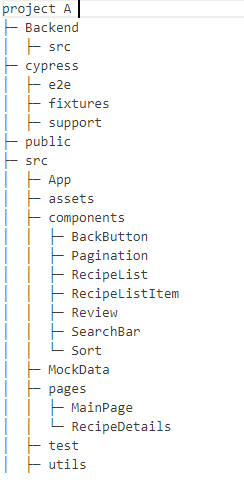
\includegraphics[width=0.30\textwidth]{Figures/A_Structure.png}\label{fig:A_stru}}
  \hfill
  \subfloat[B Structure.]{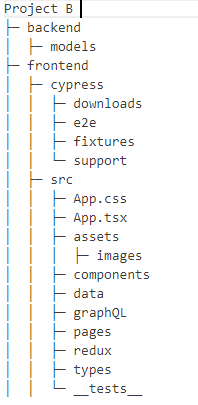
\includegraphics[width=0.29\textwidth]{Figures/B_Structure.png}\label{fig:B_Stru}}
  \hfill
  \subfloat[C Structure.]{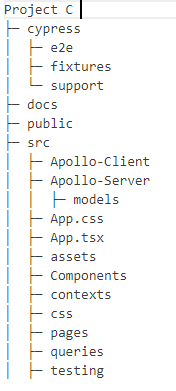
\includegraphics[width=0.27\textwidth]{Figures/C_Structure.png}\label{fig:C_Stru}}
  
\label{fig:Test_Structures}
\end{figure} \hfill 



\subsubsection{Control Project}
The control project is an open source project found on GitHub called "Hydra\footnote{https://github.com/hydralauncher/hydra}", written in TypeScript. Hydra is, as of 16.06.2024, a game launcher with 44 contributors and 1030 commits. This project serves as a control to validate the selection techniques against a larger and more complex codebase than typical student projects. By applying the selection methods to Hydra, the objective is to determine if these techniques are sufficiently accurate and inclusive when used on a substantially larger project. \\

By testing these selection techniques on both student projects and a substantially larger open-source project, the goal is to evaluate their effectiveness in different contexts. This approach aims to ensure that they provide meaningful insights and improvements to the Peer Code Review practice. \\

\noindent \textbf{Project Structure} \\
\noindent To get an overview of how the control project looks, Figure \ref{fig:Control_Structure} shows a simplified view of the project structure. Some folders are not included to make the figure readable. Only folders and sub-folders are shown. The project contained 172 files with the extensions; \textit{.ts, .js, .tsx, .jsx, .css, .html or .json}.


\begin{figure}[H]
    \centering
    \caption{Control Project structure} 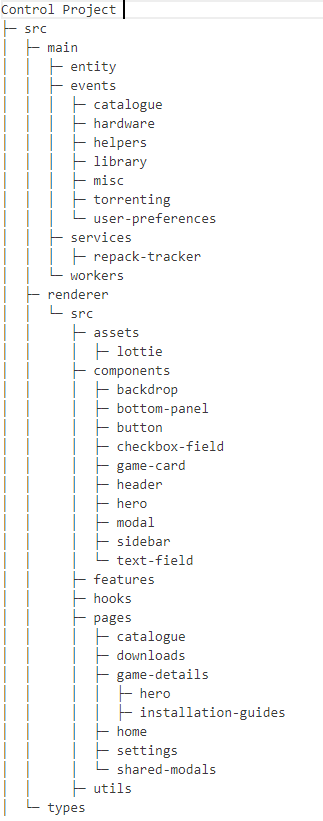
\includegraphics[width=0.3\textwidth]{Figures/Control_Structure.png}
    \label{fig:Control_Structure}
\end{figure}



\subsection{Evaluation Method}
To assess the efficiency of the various selection techniques, a controlled experiment was carried out on all the test projects, as well as the control project. Each technique was applied to the projects uniformly, which resulted in the selection of eight files by each technique for each project that, in total, resulted in 128 file selections. The files selected by each technique were then sorted into a priority list based on their metric scores. Specifically, Size Selection prioritized based on lines of code, Keyword Selection prioritized based on the occurrence of the specified keywords, Cyclomatic Complexity Selection prioritized based on the Cyclomatic Complexity score and Combination Selection prioritized based on the FTA score. During this process, the behavior of each selection technique was also observed to identify patterns or anomalies. \\

Before this, an \textit{Optimal Selection} list for each project was compiled by manually reviewing each file to determine the eight most important files for PCR. Prioritization was based on a holistic view of the project based on the logic, functionality, and complexity of the files. This meticulous process produced a benchmark list of optimal selections, which was used to assess the effectiveness and accuracy of each technique. Subsequently, comparisons were made between the files selected by each technique and the optimal selections. The consistency of each selection technique was also assessed by noting the frequency with which they identified the same files. If several selection techniques identified the same files, it suggested that these files were indeed more crucial, regardless of their inclusion in the Optimal Selection list.

%BESKRIVE DATAEN LITT GRUNDIGERE. HVA JEG HAR TESTET DET PÅ. GI LITT FAKTA. SYSTEMATISK EVALUERING MOT OPTIMAL SELECTIONS. MEN OGSÅ KJØRT EKSPERIMENTER FOR Å SE OPPFØRSELEN TIL TEKNIKKENE.
\cleardoublepage


\chapter{Results}
This chapter presents the results of the research in the thesis. For more information on how the data was collected, see Chapter \ref{Methodology}, Methodology. Firstly, optimal selections for each of the four projects will be presented to establish the benchmark for the ideal solution if the selection techniques choose perfectly. The goal is to find out which of the selection techniques; Size, Keyword, Cyclomatic Complexity, and Combination, is most effective in selecting the most important files for review.



\section{Optimal File Selection} \label{optimal_selections}
For each of the projects, there is a set of files that ideally should be selected for the technique to have made the \textit{correct} selections depending on which files are crucial to review. This is also important to ensure that the project is adequately covered in a code review. The relevant files vary for each project because they have been created by different student groups. The following subsections therefore presents the files that ideally should be selected for each technique to perform optimally. If the actual selection by the various techniques does not match the ideal selection, it could be due to several reasons. The primarily reason is, most probably, that the different selection techniques are not perfectly comprehensive and do not cover all aspects of the codebase. Additional information on the selection techniques can be found in Section \ref{Methodology}. \\

To establish a benchmark for evaluating the performance of each selection technique, I manually reviewed each of the projects to determine the optimal set of files. This process involved identifying the most crucial files that should be included in a thorough code review, considering factors such as functionality, complexity, size, critical features, and the amount of logic present. By creating a close-to-ideal selection scenario, it becomes easier to assess the strengths and weaknesses of each technique. In the following subsections, the files are presented along with the selection category they belong to. \\

This optimal selection process is based on my expertise and experience as a teaching assistant for three semesters, during which I reviewed numerous peer code submissions. The selected files are based on a combination of my understanding of the best practices in software development and my specific knowledge of the course projects. As mentioned above, the optimal selections are selected according to a combined assessment that considers functionality, complexity, size, critical features, and the amount of logic present. There is a degree of subjectivity in this selection, since it is merely my subjective opinions deciding what are crucial files to include. However, it provides an arguably reasonable standard that the automated selection techniques can be compared against. This selection process was completed before applying the various techniques to the projects so as not to be affected by their results and to keep the selection unbiased. \\

By comparing the files selected by each technique with this ideal set, we can identify where each method excels and where it does not suffice. This comparison will highlight the effectiveness of the different selection strategies in capturing the most crucial parts of the codebase, and will ensure that key functionalities are adequately reviewed. This analysis will provide valuable information on the practical application of these techniques in educational contexts.

\subsection{Project A - Optimal Selections}
For project A, the optimal selections are, ordered as they appear in the project, as follows: \\ 


\begin{center}
\begin{tabularx}{\textwidth}{>{\hsize=1.1\hsize}X >{\hsize=0.9\hsize}X}
    \toprule
    \textbf{Path} & \textbf{Selection Category} \\
    \midrule
    \texttt{src/resolvers.ts} & Functionality, Logic, Complexity  \\   
    \texttt{components/RecipeList/index.tsx} & Functionality, Logic, Complexity \\
    \texttt{components/RecipeListItem/index.tsx} & Logic \\   
    \texttt{components/Review/index.tsx} & Logic, Complexity \\
    \texttt{components/SearchBar/index.tsx} & Functionality \\
    \texttt{pages/MainPage/index.tsx} & Functionality,  Logic, Complexity \\
    \texttt{pages/RecipeDetails/index.tsx} & Functionality, Complexity \\
    \texttt{utils/GlobalContext.tsx} & Functionality, Logic\\
    \bottomrule
    
\end{tabularx}
\end{center}

\subsection{Project B - Optimal Selections}
For project B, the optimal selections are, ordered as they appear in the project, as follows: \\ 


\begin{center}
\begin{tabularx}{\textwidth}{>{\hsize=1.1\hsize}X >{\hsize=0.9\hsize}X}
    \toprule
    \textbf{Path} & \textbf{Selection Category} \\
    \midrule
    \texttt{backend/resolvers.ts} & Functionality,  Logic, Complexity  \\
    \texttt{components/DropdownMenu.tsx} & Logic, Complexity  \\
    \texttt{components/FavoriteButton.tsx} & Logic, Complexity  \\
    \texttt{components/Header.tsx} & Logic  \\
    \texttt{components/ReviewSection.tsx} & Functionality,  Logic, Complexity  \\
    \texttt{pages/Carpage.tsx} & Functionality,  Logic, Complexity  \\
    \texttt{pages/Filterpage.tsx} & Functionality,  Logic, Complexity  \\ 
    \texttt{pages/Homepage.tsx} & Functionality,  Logic  \\
    \bottomrule
\end{tabularx}
\end{center}


\subsection{Project C - Optimal Selections}
For project C, the optimal selections are, ordered as they appear in the project, as follows: \\ 


\noindent
\begin{center}
\begin{tabularx}{\textwidth}{>{\hsize=1.1\hsize}X >{\hsize=0.9\hsize}X}
    \toprule
    \textbf{Path} & \textbf{Selection Category} \\
    \midrule
    \texttt{Apollo-Server/index.tsx} & Functionality,  Logic, Complexity \\
    \texttt{Components/AboutWineComponent.tsx} & Functionality,  Logic, Complexity \\
    \texttt{Components/FilterComponent.tsx} & Functionality, Complexity \\
    \texttt{Components/HeaderComponent.tsx} & Functionality, Logic \\
    \texttt{Components/WineComponent.tsx} & Logic \\
    \texttt{pages/Homepage.tsx} & Functionality,  Logic, Complexity \\
    \texttt{contexts/FavoriteContext.tsx} & Functionality, Complexity \\
    \texttt{contexts/SearchContext.tsx} & Functionality \\
    \bottomrule
\end{tabularx}
\end{center}


\subsection{Control project - Optimal Selections}
For the control project, I could not confidently identify which files were more critical compared to the others, as it was such a complex project. Therefore, the files for these optimal selections are based solely on the various techniques. The comparison for this project in the discussion will not be compared to an optimal solution but instead will be all the selection techniques compared against each other for a joint comparison.\\




\section{Results for Each Selection Technique}
In this section, I will present the results for each of the file selections for each of the projects when applied with the different selection techniques. These selection techniques, presented in Section \ref{Methodology}, include Size Selection, Keyword Selection, Cyclomatic Complexity Selection, and Combination Selection. The results will highlight how well each technique identifies critical code segments and whether it aligns with the optimal selections presented in Section \ref{optimal_selections}. The files selected for each project will be visualized and then briefly described. This visualization will provide a detailed view of their performance. \\

To be able to visualize the results in a clear and organized manner, some adjustments have been made to the way the names of various files in the tables in this section are displayed. The files have been renamed to reflect the name of the folder above the file in the project hierarchy. For example, in table \ref{tab:Selected_files_A}, the name of \textit{Mainpage/index.tsx} has been changed to \textit{Mainpage.tsx}. For project C, some of the files with names containing "Component", have been renamed without that part. For example \textit{AboutWineComponent.tsx} to \textit{AboutWine.tsx}. This has no functional impact on the results or the thesis, but is solely to improve the presentation in the report.


\subsection{Project A Results}
For project A, the Keyword Selection technique only selected 7 files, although the specification was to select the 8 most crucial files. This is because the keywords selected to be searched for, which are introduced in Section \ref{Methodology}, only appeared in 7 of the files in the project. 


\begin{figure}[H]
  \centering
  \caption[Project A Selections and Metrics]{For each figure, the path to the selected file and the data point used to make the selection is shown. Figure (a) shows the files selected by the Size Selection technique, figure (b) shows the files selected by the Keyword Selection technique, figure (c) shows the files selected by the Cyclomatic Complexity Selection technique and figure (d) shows the files selected by the Combination Selection technique.}
  \subfloat[Selected files by Size Selection.]{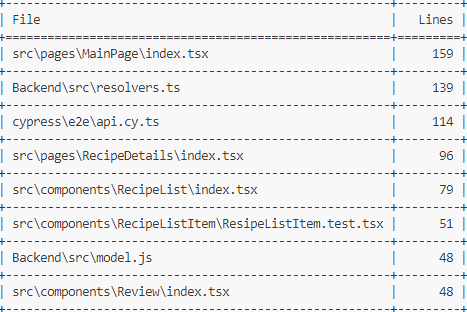
\includegraphics[width=0.49\textwidth]{Figures/A_Size.png}\label{fig:A_Size}}
  \hfill
  \subfloat[Selected files by Keyword Selection.]{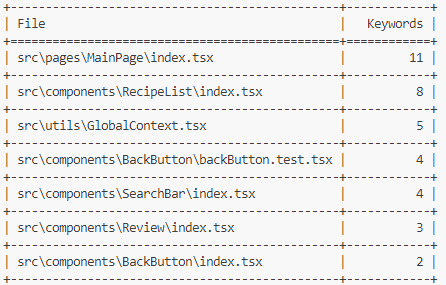
\includegraphics[width=0.46\textwidth]{Figures/A_Keyword.png}\label{fig:A_Keyword}}
  \hfill
  \subfloat[Selected files by Cyclomatic Complexity Selection.]{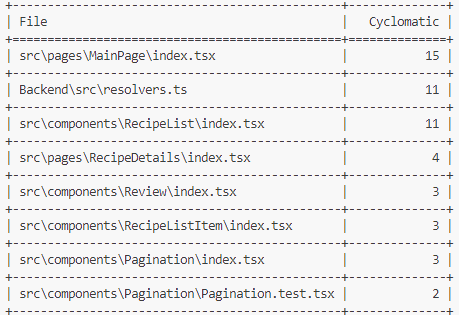
\includegraphics[width=0.49\textwidth]{Figures/A_Cyclomatic.png}\label{fig:A_Cyclomatic}}
  \hfill
  \subfloat[Selected files by Combination Selection.]{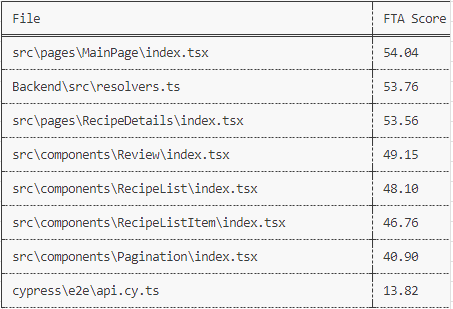
\includegraphics[width=0.49\textwidth]{Figures/A_Combination.png}\label{fig:A_Combination}}
  
\label{fig:Aresults}
\end{figure} \hfill 

The selected files by each technique have some overlap, which is both expected and a good indication that more than one selection technique effectively identifies crucial files.
The metric used by \textbf{Size Selection} selected files ranging from 159 to 48 lines of code (LOC), meaning that the following files after the 8 selected by this technique had equal or even fewer LOC and therefore probably had less relevance for being selected for review.
The metric selected for \textbf{Keyword Selection} were "useState", "useEffect", and "useNavigate", and were present in 7 of the files in project A. This metric ranged from 11 cases in \textit{Mainpage.tsx} to 2 cases in \textit{BackButton.tsx}.
The \textbf{Cyclomatic Complexity} metric ranged from a score of 15 in \textit{Mainpage.tsx} to 2 in \textit{Pagination.test.tsx}.
In the results from \textbf{Combination Selection}, the FTA scores ranged from 54.04 in \textit{Mainpage.tsx} to 13.82 in \textit{Pagination.tsx}. However, it should be noted that the seventh selection in the Combination Selection had an FTA score of 40.90. This indicates that the first 7 files selected by this technique covered the most problematic files which subsequently would be the most relevant ones for review. \\

Table \ref{tab:Selected_files_A} below visualizes the files selected by each technique with colors showing the corresponding selections between the different selection techniques.

\begin{table}[h!]
  \centering
  \fontsize{10}{10}\selectfont
  \caption{Comparison of selected files for project A by each technique}
  \label{tab:Selected_files_A}
  \begin{tabularx}{\textwidth}{llll}
    \hline
     \textbf{Size} & \textbf{Keyword} & \textbf{Cyclomatic } & \textbf{Combination} \\
     \textbf{} & \textbf{} & \textbf{Complexity } & \textbf{} \\ [1ex] \hline \hline 
    \colorbox{BurntOrange}{Mainpage.tsx} & \colorbox{BurntOrange}{MainPage.tsx} & \colorbox{BurntOrange}{MainPage.tsx} & \colorbox{BurntOrange}{MainPage.tsx} \\ [2ex]
    \colorbox{Tan}{resolvers.ts} & \colorbox{PineGreen}{RecipeList.tsx} & \colorbox{Tan}{resolvers.ts} & \colorbox{Tan}{resolvers.ts} \\ [2ex]
    \colorbox{WildStrawberry}{api.cy.ts} & GlobalContext.tsx & \colorbox{PineGreen}{RecipeList.tsx} & \colorbox{CornflowerBlue}{RecipeDetails.tsx} \\ [2ex]
    \colorbox{CornflowerBlue}{RecipeDetails.tsx} & backButton.test.tsx & \colorbox{CornflowerBlue}{RecipeDetails.tsx} & \colorbox{Rhodamine}{Review.tsx} \\ [2ex] 
    \colorbox{PineGreen}{RecipeList.tsx} & SearchBar.tsx & \colorbox{Rhodamine}{Review.tsx} & \colorbox{PineGreen}{RecipeList.tsx} \\ [2ex] 
    ResipeListItem.test.tsx & \colorbox{Rhodamine}{Review.tsx} & \colorbox{Mulberry}{RecipeListItem.tsx} & \colorbox{Mulberry}{RecipeListItem.tsx} \\ [2ex] 
    model.js & Backbutton.tsx & \colorbox{LimeGreen}{Pagination.tsx} & \colorbox{LimeGreen}{Pagination.tsx} \\ [2ex]
    \colorbox{Rhodamine}{Review.tsx} & ----------------- & Pagination.test.tsx & \colorbox{WildStrawberry}{api.cy.ts} \\ [2ex] 

  \end{tabularx}
\end{table}


For project A, the different techniques had some overlap in the selected files. All techniques selected \textit{MainPage.tsx} as the most critical file to be reviewed. After this, only Keyword Selection did not have \textit{resolvers.ts} as the second most crucial; in fact, this file was not present in its selections at all. \\

From here, the various techniques started differentiating more in the ordering of importance of files for review. However, the selected files by Size, Cyclomatic Complexity, and Combination Selection were about the same with a few exceptions. These were that Size Selection was the only technique that selected \textit{ResipeListItem.test.tsx} and \textit{model.js}, while Cyclomatic Complexity Selection was the only technique that selected \textit{Pagination.test.tsx}. \\

Combination Selection was the only technique that had all its files selected by at least one other technique, while Keyword Selection had the most files solely selected by this technique. There were two files selected uniquely by Size Selection that were not selected by any other technique. This applied to four files for Keyword Selection and one file for Cyclomatic Complexity.



\newpage
\subsection{Project B Results} 
The selections for each technique applied in project B are shown in Figure \ref{fig:Bresults}. 

\begin{figure}[H]
  \centering
  \caption[Project B Selections and Metrics]{For each figure, the path to the selected file and the data point used to make the selection is shown. Figure (a) shows the files selected by the Size Selection technique, figure (b) shows the files selected by the Keyword Selection technique, figure (c) shows the files selected by the Cyclomatic Complexity Selection technique and figure (d) shows the files selected by the Combination Selection technique.}
  \subfloat[Selected files by Size Selection.]{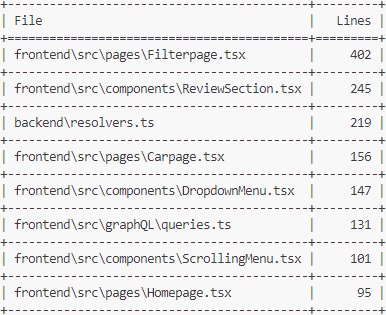
\includegraphics[width=0.47\textwidth]{Figures/B_Size.png}\label{fig:B_Size}}
  \hfill
  \subfloat[Selected files by Keyword Selection.]{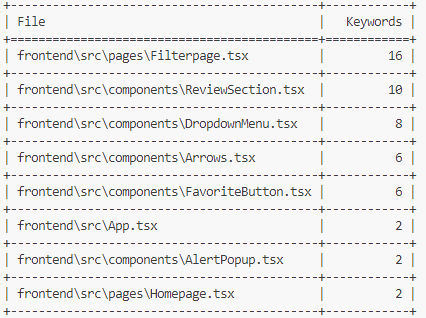
\includegraphics[width=0.51\textwidth]{Figures/B_Keyword.png}\label{fig:B_Keyword}}
  \hfill
  \subfloat[Selected files by Cyclomatic Complexity Selection.]{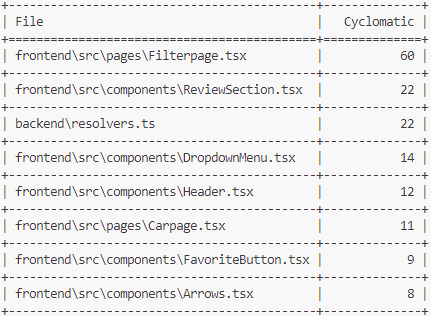
\includegraphics[width=0.49\textwidth]{Figures/B_Cyclomatic.png}\label{fig:B_Cyclomatic}}
  \hfill
  \subfloat[Selected files by Combination Selection.]{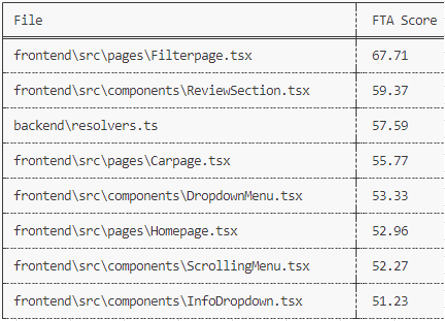
\includegraphics[width=0.49\textwidth]{Figures/B_Combination.png}\label{fig:B_Combination}}
  
\label{fig:Bresults}
\end{figure} \hfill 

Similarly as with project A, the selected files by each technique have some overlap, which was both expected, and also a good indication that more than one selection technique effectively identifies which files are crucial. 
For project B, the metric used by \textbf{Size Selection} selected files that ranged from 402 to 95 lines of code (LOC). This is a larger gap than for project A. In addition, the eighth file having 95 LOC could indicate that the following files after this would also have code that might be necessary to include in a review.
The metrics selected for \textbf{Keyword Selection} were present in 9 of the files in project B. This metric ranged from 16 cases in \textit{Filterpage.tsx} to 2 cases in \textit{Homepage.tsx}.
The \textbf{Cyclomatic Complexity} metric ranged from a score of 60 in \textit{Filterpage.tsx} to 8 in \textit{Arrows.tsx}. This represents a significant increase compared to project A, which had a Cyclomatic Complexity score of 15 in \textit{Mainpage.tsx}.
In the results from the \textbf{Combination Selection}, the FTA scores ranged from 67.71 in \textit{Filterpage.tsx} to 51.23 in \textit{InfoDropdown.tsx}. After the 15th file selection with Combination Selection, the FTA score went from 46.43 in one file to 12.73 for the next.


\begin{table}[h!]
  \centering
  \fontsize{10}{10}\selectfont
  \caption{Comparison of selected files for project B by each technique}
  \label{tab:Selected_files_B}
  \begin{tabularx}{\textwidth}{llll}
    \hline
     \textbf{Size} & \textbf{Keyword} & \textbf{Cyclomatic } & \textbf{Combination} \\
     \textbf{} & \textbf{} & \textbf{Complexity } & \textbf{} \\ [1ex] \hline \hline 
    \colorbox{BurntOrange}{Filterpage.tsx} & \colorbox{BurntOrange}{Filterpage.tsx} & \colorbox{BurntOrange}{Filterpage.tsx} & \colorbox{BurntOrange}{Filterpage.tsx} \\ [2ex]
    \colorbox{Tan}{ReviewSection.tsx} & \colorbox{Tan}{ReviewSection.tsx} & \colorbox{Tan}{ReviewSection.tsx} & \colorbox{Tan}{ReviewSection.tsx} \\ [2ex]
    \colorbox{CornflowerBlue}{resolvers.ts} & \colorbox{PineGreen}{DropdownMenu.tsx} & \colorbox{CornflowerBlue}{resolvers.ts} & \colorbox{CornflowerBlue}{resolvers.ts} \\ [2ex]
    \colorbox{Rhodamine}{Carpage.tsx} & \colorbox{WildStrawberry}{Arrows.tsx} & \colorbox{PineGreen}{DropdownMenu.tsx} & \colorbox{Rhodamine}{Carpage.tsx} \\ [2ex] 
    \colorbox{PineGreen}{DropdownMenu.tsx} & \colorbox{Orchid}{FavoriteButton.tsx} & Header.tsx & \colorbox{PineGreen}{DropdownMenu.tsx} \\ [2ex] 
    queries.ts & App.tsx & \colorbox{Rhodamine}{Carpage.tsx} & \colorbox{Mulberry}{Homepage.tsx} \\ [2ex] 
    \colorbox{LimeGreen}{ScrollingMenu.tsx} & AlertPopup.tsx & \colorbox{Orchid}{FavoriteButton.tsx} & \colorbox{LimeGreen}{ScrollingMenu.tsx} \\ [2ex]
    \colorbox{Mulberry}{Homepage.tsx} & \colorbox{Mulberry}{Homepage.tsx} & \colorbox{WildStrawberry}{Arrows.tsx} & InfoDropdown.tsx \\ [2ex] 

  \end{tabularx}
\end{table}

Also in project B there was overlap in the most crucial files identified by each technique. All selection techniques had selected the two same files as the most crucial and second most crucial. These files were \textit{Filterpage.tsx} and \textit{ReviewSection.tsx} respectively. All techniques had also selected \textit{DropdownMenu.tsx}, but with a difference in the ordering of importance. \\

After this point, the various techniques had some overlap with other techniques in most of the selections. Size Selection and Combination Selection had the most in common, with both having only one selection, which the other did not. Keyword Selection and Cyclomatic Complexity Selection also had more selections in common than the other two. They had two file selections in common that the other techniques did not select, specifically \textit{Arrows.tsx} and \textit{FavoriteButtion.tsx}. \\

For project B, all the selection techniques had at least one selection that no other technique had selected. For Size Selection it was \textit{queries.ts}, for Keyword Selection it was \textit{App.tsx} and \textit{AlertPopup.tsx}, for Cyclomatic Complexity Selection it was \textit{Header.tsx} while for Combination Selection it was \textit{InfoDropdown.tsx}. \\




\subsection{Project C Results} 

\begin{figure}[H]
  \centering
  \caption[Project C Selections and Metrics]{For each figure, the path to the selected file and the data point used to make the selection is shown. Figure (a) shows the files selected by the Size Selection technique, figure (b) shows the files selected by the Keyword Selection technique, figure (c) shows the files selected by the Cyclomatic Complexity Selection technique and figure (d) shows the files selected by the Combination Selection technique.}
  \subfloat[Selected files by Size Selection.]{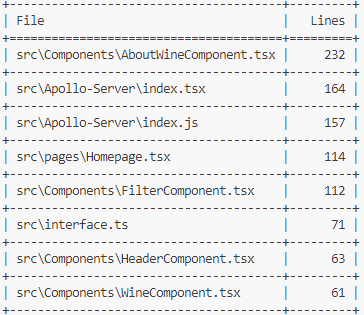
\includegraphics[width=0.48\textwidth]{Figures/C_Size.png}\label{fig:C_Size}}
  \hfill
  \subfloat[Selected files by Keyword Selection.]{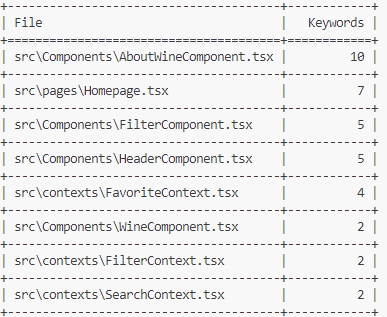
\includegraphics[width=0.50\textwidth]{Figures/C_Keyword.png}\label{fig:C_Keyword}}
  \hfill
  \subfloat[Selected files by Cyclomatic Complexity Selection.]{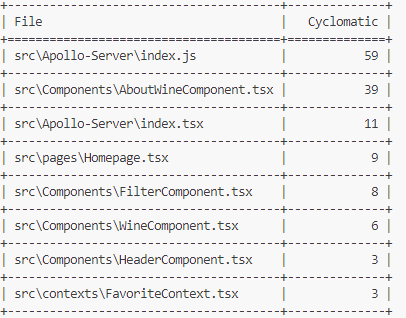
\includegraphics[width=0.51\textwidth]{Figures/C_Cyclomatic.png}\label{fig:C_Cyclomatic}}
  \hfill
  \subfloat[Selected files by Combination Selection.]{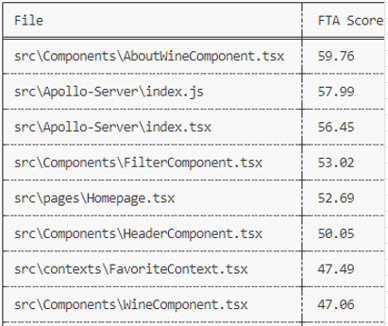
\includegraphics[width=0.48\textwidth]{Figures/C_Combination.png}\label{fig:C_Combination}}
  
\label{fig:Cresults}
\end{figure} \hfill 

In project C, the metric used by \textbf{Size Selection} selected files ranging from 232 LOC to 61 LOC. This is more similar to the gap found in project A. However, since the eighth file had 61 LOC, it is possible that there are crucial files below this threshold as well that were excluded selection.
In this project, \textbf{Keyword Selection} found the selected keywords in 10 files. These cases ranged from 10 occurrences in \textit{AboutWine.tsx} to two occurrences in \textit{Favoritepage.tsx}.
\textbf{Cyclomatic Complexity Selection} ranged from a score of 59 in \textit{Apollo-Server.tsx} to a score of three in \textit{FavoriteContext.tsx}. This was similar to the result from applying this technique on project B, but in this instance it selected all the files with a score above three instead.
The \textbf{Combination Selection} had files selected with scores ranging from 59.76 to 47.06 in \textit{AboutWine.tsx} to \textit{Wine.tsx} respectively. The FTA score dropped to 12.56 with the file following \textit{Wine.tsx}, indicating that the first eight files clearly were the most crucial ones. \\


\begin{table}[H]
  \centering
  \fontsize{10}{10}\selectfont
  \caption{Comparison of selected files for project C by each technique}
  \label{tab:Selected_files_C}
  \begin{tabularx}{\textwidth}{llll}
    \hline
     \textbf{Size} & \textbf{Keyword} & \textbf{Cyclomatic } & \textbf{Combination} \\
     \textbf{} & \textbf{} & \textbf{Complexity } & \textbf{} \\ [1ex] \hline \hline 
    \colorbox{BurntOrange}{AboutWine.tsx} & \colorbox{BurntOrange}{AboutWine.tsx} & \colorbox{Tan}{Apollo-Server.js} & \colorbox{BurntOrange}{AboutWine.tsx} \\ [2ex]
    \colorbox{CornflowerBlue}{Apollo-Server.tsx} & \colorbox{Rhodamine}{Homepage.tsx} & \colorbox{BurntOrange}{AboutWine.tsx} & \colorbox{Tan}{Apollo-Server.js} \\ [2ex]
    \colorbox{Tan}{Apollo-Server.js} & \colorbox{PineGreen}{Filter.tsx} & \colorbox{CornflowerBlue}{Apollo-Server.tsx} & \colorbox{CornflowerBlue}{Apollo-Server.tsx} \\ [2ex]
    \colorbox{Rhodamine}{Homepage.tsx} & \colorbox{LimeGreen}{Header.tsx} & \colorbox{Rhodamine}{Homepage.tsx} & \colorbox{PineGreen}{Filter.tsx} \\ [2ex] 
    \colorbox{PineGreen}{Filter.tsx} & \colorbox{Orchid}{FavoriteContext.tsx} & \colorbox{PineGreen}{Filter.tsx} & \colorbox{Rhodamine}{Homepage.tsx} \\ [2ex] 
    interface.ts & \colorbox{Mulberry}{Wine.tsx} & \colorbox{Mulberry}{Wine.tsx} & \colorbox{LimeGreen}{Header.tsx} \\ [2ex] 
    \colorbox{LimeGreen}{Header.tsx} & FilterContext.tsx & \colorbox{LimeGreen}{Header.tsx} & \colorbox{Orchid}{FavoriteContext.tsx} \\ [2ex]
    \colorbox{Mulberry}{Wine.tsx} & SearchContext.tsx & \colorbox{Orchid}{FavoriteContext.tsx} & \colorbox{Mulberry}{Wine.tsx} \\ [2ex] 

  \end{tabularx}
\end{table}

Project C is the one with the most crucial file selection overlap of the three test projects. As seen in Table \ref{tab:Selected_files_C}, there are only three selected files that were selected by a single technique. These files were \textit{interface.ts} which got selected by Size Selection, and \textit{FilterContext.tsx} and \textit{SearchContext.tsx} which got selected by Keyword Selection. All remaining selected files were selected by at least one other technique. \\

Size, Cyclomatic Complexity, and Combination Selection all selected the same files as the 5 most crucial files. However, they all had different placements in the order of importance. The only similar ordering was \textit{Homepage.tsx} and \textit{Filter.tsx} for Size and Cyclomatic Complexity, and \textit{Apollo-Server.tsx} for Cyclomatic Complexity and Combination. \\

For this project, Cyclomatic Complexity Selection and Combination Selection had selected all the same files, just with different ordering. Size Selection selected one different file, which exempted it from having identical selections to Cyclomatic Complexity and Combination. \\



\subsection{Control Project Results} 
The control project serves as a benchmark to evaluate the performance of each selection technique on a larger and more complex codebase. The following subsection details the results of applying each technique in this project.

\begin{figure}[H]
  \centering
  \caption[Control Project Selections and Metrics]{For each figure, the path to the selected file and the data point used to make the selection. Figure (a) shows the files selected by the Size Selection technique, figure (b) shows the files selected by the Keyword Selection technique, figure (c) shows the files selected by the Cyclomatic Complexity Selection technique and figure (d) shows the files selected by the Combination Selection Technique.}
  \subfloat[Selected files by Size Selection.]{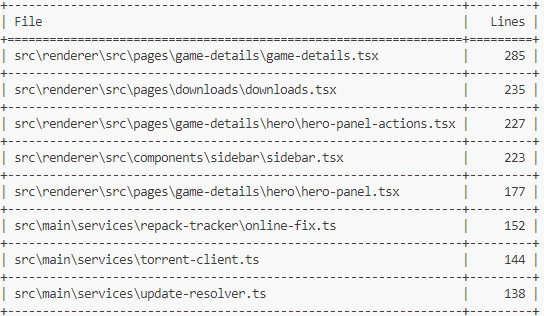
\includegraphics[width=0.48\textwidth]{Figures/Control_Size.png}\label{fig:Control_Size}}
  \hfill
  \subfloat[Selected files by Keyword Selection.]{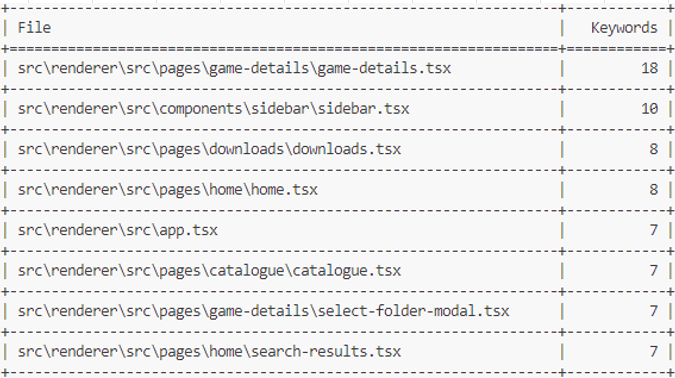
\includegraphics[width=0.48\textwidth]{Figures/Control_Keyword.png}\label{fig:Control_Keyword}}
  \hfill
  \subfloat[Selected files by Cyclomatic Complexity Selection.]{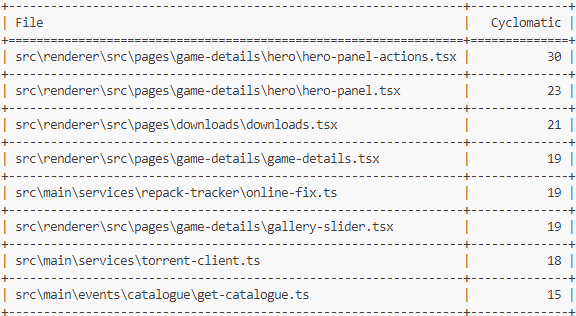
\includegraphics[width=0.54\textwidth]{Figures/Control_Cyclomatic.png}\label{fig:Control_Cyclomatic}}
  \hfill
  \subfloat[Selected files by Combination Selection.]{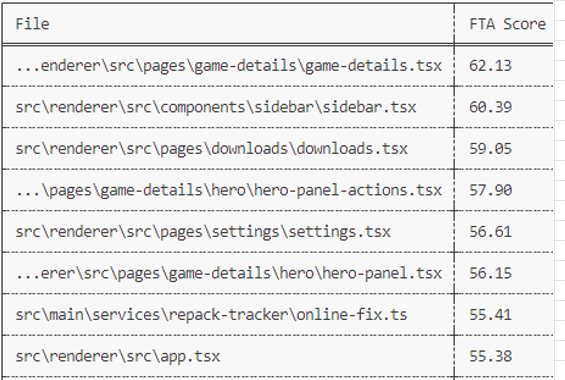
\includegraphics[width=0.44\textwidth]{Figures/Control_Combination.png}\label{fig:Control_Combination}}
  \label{fig:Controlresults}
\end{figure}

We can see that the selected files for each technique have some overlap, although not as much as the test projects. This is not surprising, as the codebase in this control project is both bigger and more complex than the test projects.
The \textbf{Size Selection} technique this time selected files with metrics ranging from 285 lines of code in \textit{game-details.tsx} to 138 lines of code in \textit{update-resolver.ts}. 
As a substantially larger project, this time the \textbf{Keyword Selection} found keywords in 22 files, which is more than twice the amount found in any test project. The occurrences ranged from 18 in \textit{game-details.tsx} to 7 occurrences in \textit{search-result.tsx}, and down to 2 in the least prioritized file.
The \textbf{Cyclomatic Complexity Selection} metric ranged from 30 in \textit{hero-panel-actions.tsx} to a score of 15 in \textit{get-catalogue.tsx}. 
\textbf{Combination Selection} this time ranged from a FTA score in \textit{game-details.tsx} of 62.13 to \textit{app.tsx} with a FTA score of 55.38. In the control project, the FTA score was above 30 all the way until the 55th file selection, then it dropped to 14 and below. This indicates that most of the files until this 55th file could be relevant to include in a review. \\


\begin{table}[H]
  \centering
  \caption{Comparison of selected files for control project by each technique}
  \label{tab:Selected_files_control}
  \begin{tabularx}{\textwidth}{llll}
    \hline
     \textbf{Size} & \textbf{Keyword} & \textbf{Cyclomatic } & \textbf{Combination} \\
     \textbf{} & \textbf{} & \textbf{Complexity } & \textbf{} \\ [1ex] \hline \hline 
    \colorbox{BurntOrange}{game-details.tsx} & \colorbox{BurntOrange}{game-details.tsx} & \colorbox{Rhodamine}{hero-actions.tsx} & \colorbox{BurntOrange}{game-details.tsx} \\ [2ex]
    \colorbox{Tan}{downloads.tsx} & \colorbox{CornflowerBlue}{sidebar.tsx} & \colorbox{PineGreen}{hero-panel.tsx} & \colorbox{CornflowerBlue}{sidebar.tsx} \\ [2ex]
    \colorbox{Rhodamine}{hero-actions.tsx} & \colorbox{Tan}{downloads.tsx} & \colorbox{Tan}{downloads.tsx} & \colorbox{Tan}{downloads.tsx} \\ [2ex]
    \colorbox{CornflowerBlue}{sidebar.tsx} & home.tsx & \colorbox{BurntOrange}{game-details.tsx} & \colorbox{Rhodamine}{hero-actions.tsx} \\ [2ex] 
    \colorbox{PineGreen}{hero-panel.tsx} & \colorbox{WildStrawberry}{app.tsx} & \colorbox{Mulberry}{online-fix.ts} & settings.tsx \\ [2ex] 
    \colorbox{Mulberry}{online-fix.ts} & catalogue.tsx & gallery-slider.tsx & \colorbox{PineGreen}{hero-panel.tsx} \\ [2ex] 
    \colorbox{LimeGreen}{torrent-client.ts} & select-modal.tsx & \colorbox{LimeGreen}{torrent.client.ts} & \colorbox{Mulberry}{online-fix.ts} \\ [2ex]
    update-resolver.ts & search-results.tsx & get-catalogue.ts & \colorbox{WildStrawberry}{app.tsx} \\ [2ex] 

  \end{tabularx}
\end{table}

In the control project, there were more notable differences between the various techniques than in the test projects. Although, there was still some overlap in the selections, such as all techniques choosing \textit{game-details.tsx} and \textit{downloads.tsx} among the most important files. However, Cyclomatic Complexity stood out in this by indicating that \textit{downloads.tsx} was more important than \textit{game-details.tsx}. At the same time, the other three techniques had chosen \textit{sidebar.tsx} among the most important files, while Cyclomatic Complexity did not select it. \\

Keyword Selection had the most different selections compared to the other techniques, with only 4 out of 8 files being chosen by at least one other technique. It did not select files such as \textit{hero-panel-actions.tsx}, \textit{online-fix.tsx}, and \textit{hero-panel.tsx}, which the other three techniques all selected. \\

The Control Project and Project C were the projects in which all techniques had selected at least one file exclusively that none of the other techniques had selected. For this project, it was one file for Size Selection, four files for Keyword Selection, two files for Cyclomatic Complexity Selection, and one file for Combination Selection.
\cleardoublepage


\chapter{Conclusion}
To address problems and inefficiencies with Peer Code Reviews in education, the objective of this thesis was to find out what selection techniques perform best to select crucial code to put in a review. This was done by a controlled experiment with a set of optimal files already known for each project. Eight files were selected by each technique for each of the three test projects and the control project. The results of the experiment will now be discussed. \\

The findings indicate that all selection techniques are efficient in identifying many of the files that are crucial in a repository. However, some techniques had higher accuracy in the selection of crucial files, while other techniques were more consistent in their selection. The \textbf{Keyword Selection} technique is unique, as this technique could vary greatly depending on what keywords are used to identify the files and therefore has a more focused selection than the rest. \\

\noindent The objective of the thesis reads as follows:
\begin{quote}
    \textit{Find the code selection techniques that are most effective in ensuring that the most critical code is selected for review in educational contexts, and investigate how these methods enhance the review process}
\end{quote}

To help answer this objective, this chapter will discuss how the selection techniques compare to each other, why they made the selections they did, and whether these selections were adequate. In addition, the accuracy, coverage, and consistency of the techniques will be discussed. The question of how the results reflect the research questions will also be discussed. \\



\section{Discussion}
%Hva som fungerer og hvorfor det fungerer. Vise at man skjønner systemet.

When it comes to the selection techniques, all four performed adequately for their respective metrics. However, none of the techniques made perfect selections compared to the optimal selections, which will be discussed in Section \ref{Selections_compared}. \\


\subsection{Comparison of Selections} \label{Selections_compared}
\begin{quote}
    \textbf{RQ1:} How do code selection methods compare to each other?
\end{quote}

% most reliable depending on different metrics. accuracy, consistency, coverage and overall performance?\\
In order to evaluate the selection techniques, I will consider the measures; accuracy, coverage, and consistency, based on their results on the test projects. \\

\begin{table}[H]
  \centering
  \begin{tabularx}{\textwidth}{>{\hsize=0.5\hsize}X >{\hsize=1.5\hsize}X}
    \textbf{Measure} & \textbf{Description} \\ [1ex] \hline 
    
    \textbf{Accuracy} & Determined by the degree to which the selections align with the optimal selections. \\ [1ex]
    
    \textbf{Coverage} & Depends on how comprehensively the repository/project is covered. \\ [1ex] 
    
    \textbf{Consistency} & Measured by the extent to which the selections match with the other techniques' selections. \\ \hline
  \end{tabularx}
  \caption{Evaluation measures for the selection techniques}
  \label{tab:Evaluation_Measures}
\end{table}


\subsubsection{Accuracy}
% Which method selected the most optimal files average?\\
When comparing the accuracy of all selection techniques with the optimal selections in Section \ref{optimal_selections}, several notable observations can be made. Although each technique identified a significant number of optimal file selections, none of the selection techniques achieved perfect accuracy in their selections. However, some techniques had better accuracy than others. Excluding the control project, the number of matching selections between the selection techniques and the optimal selections are shown in Table \ref{tab:Accuracy}.

\begin{table}[H]
  \centering
  \begin{tabularx}{\textwidth}{>{\hsize=1.4\hsize}X >{\hsize=0.6\hsize}X >{\hsize=0.6\hsize}X >{\hsize=0.6\hsize}X}
    \textbf{Technique} & \textbf{Project A} & \textbf{Project B} & \textbf{Project C} \\ [1ex] \hline 
    
    \textbf{Size} & 5 files & 6 files & 6 files \\ [1ex]
    
    \textbf{Keyword} & 5 files & 5 files & 7 files \\ [1ex] 
    
    \textbf{Cyclomatic Complexity} & 6 files & 7 files & 7 files \\ [1ex]
    
    \textbf{Combination} & 6 files & 6 files & 7 files \\ \hline

  \end{tabularx}
  \caption{Selected files per technique matching the optimal selections}
  \label{tab:Accuracy}
\end{table}

The average accuracy is calculated by adding, for each technique, the number of matching selections to the optimal selections together and dividing it by the number of projects. The average accuracy is therefore as follows; 5.7 for Size Selection, 5.7 for Keyword Selection, 6.3 for Combination Selection, and 6.7 for Cyclomatic Complexity Selection. This suggests that Cyclomatic Complexity was the most accurate selection technique, which is intriguing. Combination Selection is a combination of multiple techniques, which would make it natural to imply that it is more accurate since it takes more metrics into consideration when finding crucial files. The Combination Selection technique incorporates Cyclomatic Complexity along with additional measures to determine the selections, which could imply that including size or Halstead measures in the calculations may have reduced the technique's accuracy. \\

While none of the techniques got a perfect selection, there were cases where only one file was not selected from the optimal selections by techniques. Specifically Cyclomatic Complexity Selection in Project B, and all techniques except Size Selection in Project C. It also regarded some techniques in the Control Project, but this is exempt inclusion here since the optimal selections were not identified, but taken directly from the Size Selections. This means that Size Selection was the only technique that did not even get seven out of eight optimal files selected in any of the cases. As the most crucial code segments do not necessarily align with the file with most lines of code, it makes sense that this technique would have some selections that would not be optimal. This is also the case when considering the coverage of the technique. 


\subsubsection{Coverage}
Size Selection limits its coverage on the repositories by selecting based solely on lines of code. Although this measure often selects the code with the most logic or functionality, it can identify \textit{false positives} or less relevant files if it selects files with a lot of code but of little importance. This was the case in Project B where Size Selection selected \textit{queries.ts}, which contains no logic or functionality except SQL queries. This selection theoretically made sense since it had 131 lines of code, but there was no relevant functionality or code to review in this case. Because of cases like this, it is smarter to combine Size Selection with other selection techniques to negate this side effect. \\

Like Size Selection, Keyword Selection also lacks coverage, since it only searches for files containing specific keywords and does not consider other files of importance, even though these could be just as crucial to review. This is important to keep in mind if using this technique in the PCR process. While Keyword Selection lacks coverage, it still made some selections of optimal files none of the other techniques did. In Project A and C, it made respectively two and one selections of optimal selection all the other selection methods overlooked in their top eight selections. So what Keyword Selections lacks in coverage, it makes up for in relevant, focused and pinpointed selections. In Project C, if Keyword Selection and either Cyclomatic Complexity Selection or Combination Selection had been applied together, it would probably have managed to select all eight optimal files, as these techniques separately covered the optimal selections. By leveraging the strengths of multiple techniques, a more comprehensive and effective selection process could been achieved. If these techniques are utilized together, they complement each other by covering different aspects of the codebase. Combining these methods would result in selecting more than eight files initially, but by cross-referencing the selections, the most critical eight files can be identified based on their combined importance and complexity. The synergistic effect of using both techniques together leads to better coverage and accuracy in identifying files that are critical for thorough review. \\


\subsubsection{Consistency}
To measure consistency, the various selection techniques were compared with each other to obtain another relative measure of effectiveness. Compared with each other, the various techniques had significantly more matching selections than compared with the optimal selections. Combination Selection was the most consistent method, while Keyword Selection stood out as the least consistent method. The number of matching selections between the selection techniques is shown in Table \ref{tab:Consistency}

\begin{table}[H]
  \centering
  \begin{tabularx}{\textwidth}{>{\hsize=1\hsize}X >{\hsize=0.5\hsize}X >{\hsize=0.5\hsize}X >{\hsize=0.5\hsize}X >{\hsize=0.5\hsize}X}
    \textbf{Technique} & \textbf{Project A} & \textbf{Project B} & \textbf{Project C}  & \textbf{Control}\\ [1ex] \hline 
    
    \textbf{Size} & 6 files & 7 files & 7 files & 7 files \\ [1ex]
    
    \textbf{Keyword} & 3 files & 6 files & 6 files & 4 files \\ [1ex] 
    
    \textbf{Cyclomatic} & 7 files & 7 files & 8 files & 6 files \\
    \textbf{Complexity} & & & & \\ [1ex]
    
    \textbf{Combination} & 8 files & 7 files & 8 files & 7 files \\ \hline

  \end{tabularx}
  \caption{Selected files per technique matching the other techniques' selections}
  \label{tab:Consistency}
\end{table}

Combination Selection had all eight of its files selected by at least one other technique for projects A and C, and seven of the eight files for projects B and control, giving it an average consistency of 7,5. This means that its selections were consistent and close to perfect in all the projects. With such a high consistency, it is a good indicator that this technique performs the best in this measure. \\

Size Selection and Cyclomatic Complexity Selection came close with respectively 6,7 and 7,0 in average consistency. Keyword Selection in general had the most files selected that were not selected by the other techniques, with an average of 4,7. This indicates that Keyword Selection did not perform as well as the others. However, it can be explained by the specificity of the technique, which can be both an advantage and a disadvantage. Since the coverage was worse and the keywords used as metrics were limited to very specific functionality or areas of focus, it did not look for the most important files in general. This works if the course educator has a project where specific aspects is the important area to cover in a review.
The keywords in this experiment were limited to three metrics, which worked relatively well in this case. Had there been, let us say, 7 keywords used as metrics, the selections of this technique would most probably be covering more files, but the accuracy of the crucial files would most probably decrease due to larger selection. \\

A combination of Keyword Selection in conjunction with other selection techniques can therefore ensure that both crucial files are selected, but also files containing the specific functionality that might be the focus of the course which may not always contain as much complexity or lines of code as the crucial files. \\



%TENK ENKELT. VIST HVORDAN IMPLEMENTASJON KAN BLI. testet ulike teknikker som undersøker i praksis. Dra konklusjoner at de ulike teknikkene har ulike resultat og burde brukes med dette i bakhodet. 

\subsection{Educational Implementation} \label{Educational_Implementation}
\begin{quote}
    \textbf{RQ2:} How can code selection techniques be implemented in educational contexts?
\end{quote}

To address the challenges of the review process in educational contexts, a multifaceted approach is necessary. Balancing the workload and focusing on critical code files are strategies that can enhance the efficiency and effectiveness of Peer Code Reviews. Educators can develop a more practical and sustainable code review process by implementing code selection in the PCR process that will support student learning and development. \\

While all the selection techniques have some merit to them, as they all selected a significant amount of crucial files in each case, one should be aware of the shortcomings before implementing any of them in PCR. In order to get good coverage, accuracy and consistency in the selections, it is not recommended to only implement a single selection technique, as this might be lacking on several measures. My recommendation from this experiment is therefore to include at least two techniques. Combination Selection is a combination of Size, Cyclomatic Complexity and Halstead measures, but it still was not a perfect method. Applying Combination Selection with Keyword Selection on the other hand can be an improvement on coverage and consistency, and ensure a thorough selection. \\

The specific nature of a project is important to consider and might also dictate the best approach to selecting its code. If it is a project to enhance the students' knowledge on hooks and state management and navigation in web applications, Keyword Selection will likely be a relevant technique as this has a more narrow coverage and a higher focus on specific functionality, but it should be applied with another technique that has better accuracy. This is a reminder that there is not a one-size-fits-all approach to Peer Code Reviews, highlighting the importance of customizing PCR strategies to align with the specific needs of each project. \\


Reviewer fatigue is one of the most prominent challenges with code reviews and Peer Code Reviews. The files a reviewer reviews later in the process is not covered as thorough and receive less attention and comments. Since this was an experimental and controlled experiment, it was not tested on students in order to observe the effects of reviewer fatigue on the review process with selection techniques applied. However, any kind of prioritization on the files, other than the typical alphabetical ordering, that selects crucial files before less crucial files will undoubtedly positively affect the review quality since they get attention before reviewer fatigue kicks in. I am therefore inclined to declare that all the selection techniques tested in this experiment improves review quality of PCR because of less reviewer fatigue on crucial files compared to the standard tools like Gerrit and Github which uses alphabetical ordering. \\

Selection of specific files does not just combat the reviewer fatigue problem, it also ensures that the workload for students is bearable, and that they do not lose motivation and engagement during the review. By not reviewing an entire codebase, but as in this experiment just a select 8 files, the student engagement should not decrease as much, and the review quality should increase - or at least not diminish. It is difficult to say how selection techniques affect engagement without testing the selection techniques in practice and observing student learning and engagement. However, PCR with applied selection techniques is less time consuming because of fewer files to review while still focusing on the crucial and important files, which means that it is highly likely that engagement increases without negatively impacting learning or review quality. \\



\subsection{Selection Technique Implications}
\begin{quote}
    \textbf{RQ3:} What are the implications of different code selection techniques?
\end{quote}
% This question investigates how various code selection techniques affect the learning experience and outcomes. both the effectiveness of various code selection techniques and their broader educational implications. By measuring how well these techniques identify and prioritize critical code, this research will determine their overall utility and value in educational contexts.

%What patterns emerge in the different selection techniques?\\

The implications with the different selection techniques have been discussed and mentioned in various sections already but will be summarized here. Size Selection is a technique with great accuracy and consistency, but lacks on coverage and should not exclusively be utilized if used in a PCR. It is essential to balance this metric with another to avoid neglecting smaller and important files. Combining Size Selection with other techniques that consider complexity or keywords can address the limitations of relying solely on lines of code. \\

While Keyword Selection gives a focused and pinpointed approach to the selection process, it is limited by its narrow search. When searching solely for specific keywords, it is highly likely to overlook certain files that could be just as important to include but does not contain the keywords. Using Keyword Selection is therefore specifically recommended if the PCR focuses on particular areas or subjects that are essential to include in the review. Since Keyword Selection can have bias towards certain patterns, incorporating other selection techniques can balance out this limitation. \\

Cyclomatic Complexity Selection is generally a good technique and selects files with accuracy and consistency sufficient enough to be used alone. Implementing this technique in the selection process will improve its effectiveness and ensure consistency and standardization among the selections, as it is a quantitative measure. This technique can help students understand the importance of writing maintainable and understandable code. However, only focusing on areas with high complexity can lead to the oversight of important but less complex areas. \\


Combining different metrics allows for a more thorough and comprehensive review, ensuring various dimensions of complexity. Combination Selection marginally outperformed Cyclomatic Complexity Selection. That should have been expected from the beginning of the experiment, as it incorporates Size, Cyclomatic Complexity, and Halstead measures. Nevertheless, given that it only provided slightly better results, it could imply that there may be minimal unexplored differences between the two techniques, indicating that both might be close to an optimal selection approach. In educational contexts, using a combination technique can provide richer learning experiences as the students are exposed to different aspects of code complexity. As with Cyclomatic Complexity, using a combination of techniques can increase the objectivity of the review process since the metrics used are quantifiable. Using a Combination Selection, however, could present challenges if it requires the use of tools.



\section{Limitations}
There are several limitations that might have influenced the thesis to go in certain directions or introduced bias towards specific results. These limitations will be discussed in this section. \\

Since the optimal selections in Section \ref{optimal_selections} were identified by me and there was no other double-checking, there is a possibility that these are not actually the ideal selections. My expertise and experience are not perfect and can overlook certain aspects of the projects. \\

This experiment focused on testing projects written in TypeScript. Although JavaScript files and tests were included in the projects, the main focus was still TypeScript projects. Since the focus was TypeScript projects, the results might vary if the experiment is performed anew with projects written in other programming languages, since different languages have different features and complexities that could affect the results. \\

The Size, Cyclomatic Complexity, and Combination techniques have metrics that are covariant, which means they overlap in certain areas. More lines means more code, which increases the chance for more paths, or in other words, increases the Cyclomatic Complexity, and both of these are strongly related to Combination Selection.  This might have led these results to appear more consistent with each other than with Keyword Selection. \\

There was limited testing because there was no standardized template or experimental process to follow. Standardization could ensure greater consistency and reliability in the findings, reducing potential variability. If the testing had followed a standardized template and process, it might have impacted the proceedings and results. \\

The test projects were retrieved from only one project in a single course, IT2810, with the same project description. Selecting test projects from a variety of different courses and project descriptions could have produced different results. This uniformity might have led to biased results in this specific case, with the specific guidelines provided by the course professor. The control project could also have been selected using more standardized criteria, to make sure it had more in common with the test projects.\\

Lastly, the testing was performed exclusively within a programming environment (IDE), without involving any testing from students or developers. This limited testing might have narrowed down the results. A better approach would have included having a group of students perform Peer Code Reviews on projects both, without any selection technique and with the various selection techniques applied to the projects. Afterwards, the students would give feedback on the entire process. They would also answer a questionnaire covering different metrics such as perceived usefulness, perceived learning outcome, perceived review quality, and data about the comprehensiveness of bug detection and code quality feedback. This approach could have provided more comprehensive insight and a better understanding of how the selection of crucial code files in a review process impact review quality and the student motivation and learning benefits.


\section{Findings}
To find out which code selection methods are most effective in ensuring that the most critical code is reviewed, a literature review and an experiment were performed. The literature review gives an overview of how Peer Code Review is situated in today's educational and industrial era. PCR is an essential component in modern educational contexts, and focuses on knowledge sharing, learning outcomes and fostering team collaboration more than ever before. While there are still challenges with modern code reviews such as reviewer fatigue, tool limitations and reviewer expertise, its efficiency is ever-growing when the process gets more effective preparation and a more practical review process. \\

The chosen selection methods for the experiment were Size, Keyword, Cyclomatic Complexity and Combination Selection. All techniques have unique metrics and measures to compute which files are most crucial and should be included in a review. The techniques were applied to three projects from the IT2810 course with the same project description and one open source TypeScript project. To evaluate the techniques, the results were compared with a set of optimal selections for each project, as well as compared to each other. \\

The findings show that every technique had varied results, but they all selected a significant number of optimal files. Although none of the techniques had perfect accuracy, the average accuracy of eight files was 5.7 for Size Selection, 5.7 for Keyword Selection, 6.3 for Combination Selection, and 6.7 for Cyclomatic Complexity Selection. The Size Selection and Keyword Selection techniques lack coverage compared to the two other techniques, since their selection metrics could be skewed and give false positives. Combination Selection was the technique that had the best consistency when all the techniques were compared with each other. Across the four projects tested on, the Combination technique's selections were always chosen by at least one other technique, except for one file in project B and one in the Control project. \\

A combination of more techniques, or at least more than that used in the Combination Selection in this thesis, could have worked even better. This Combination technique only combined Size, Cyclomatic Complexity and Halstead measures, which still resulted in an imperfect selection. Keyword Selection showed great promise, but lacked coverage and consistency. If used in conjunction with other techniques, it could perform the best in an educational context where the learning outcome is defined and certain keywords are more relevant to review to reach the learning goal of the course. However, it remains unclear whether the arbitrarily amalgamation of techniques will yield better results. The integration of an effective technique with an ineffective one does not inherently guarantee better selection results. There are many considerations to make, and it is important to reflect on the optimal method of technique combination before proceeding with the process. Solely using Size Selection or Keyword Selection is also not recommended, since these techniques alone can come up short, but if combined with a technique like Cyclomatic Complexity or Halstead measures, it becomes more reliable. \\


%Summarize the strengths and weaknesses of each technique and suggest scenarios where one might be preferred over the others.


\section{Future work}
The findings of this thesis suggest that the inclusion of selection techniques in the Peer Code Review process improves the efficiency, engagement and lessens the workload for students. However, there are still areas that need to be explored further. Therefore, looking at the educational effect of selective review in PCR by performing experiments with student targets to observe the effect of selection techniques on motivation, engagement, review quality, and learning outcome can be interesting. This could also be done to observe the effect of reviewer fatigue and workload on projects with selection techniques applied compared to projects without them. \\

Another direction is to explore whether it is possible and even more efficient to select certain code segments from repository files rather than the whole file for review. Thus, increasing the focus of the review even further and eliminating review on unnecessary code segments. This will focus solely on the areas that are crucial, such as logic, functionality, and improved learning outcome. A possible negative impact this direction can have is that the holistic picture is dissolved even further and the learning outcome can become skewed because the reviewer does not see the bigger picture. \\

Defining a standardized experimental design to ensure future research follows the same template can be an important step to improve the research on the PCR topic. This would involve that certain conditions must be met when experimenting with selection techniques, involving student testing, etc. Having a standardized template to follow will ensure that different research can be compared and will promote better consistency in results and findings. \\

There are various selection techniques that can be explored in future research to expand the horizon of which methods and combinations of methods yield the best selection results. These techniques could be; change frequency, bug history, dependency and code smells. It is important to be aware that some of these techniques, such as change frequency and bug history, are less relevant in educational contexts. In these contexts, there often is no history to compare code to, since it often is just one delivery with the complete codebase. \\

As mentioned in Section \ref{Educational_Implementation}, applying Combination Selection with Keyword Selection could be an improvement on coverage and consistency, and ensure a thorough selection. How to properly combine these techniques and ensure they are weighed appropriately in conjunction is an interesting direction to research further, and could provide a more thorough selection technique.


%Include a section about what should or could be done in future research or explain any recommended next steps based on the results you got. This should be the last section in the discussion. \\

%Further Studies: Propose further empirical studies to verify these findings in a broader range of projects and environments. Research could specifically focus on developing and testing new metrics or combinations of metrics that might yield better coverage and accuracy.

%Experimental Validation: Suggest experimental setups where different selection techniques are applied in controlled environments to directly compare their effectiveness in identifying critical code issues.



\cleardoublepage


\addcontentsline{toc}{chapter}{\protect\numberline{}References}
\printbibliography[title={References}] %you may change the title in the toc here if you want
\cleardoublepage


\chapter*{\LARGE \textbf{Appendices}}
\fancyhf{} %clear the header, it should be empty for the appendices
\renewcommand{\headrulewidth}{0pt} %no rule
\fancyfoot[C]{\thepage} %set the page numbers in the center of the footer instead 

%it is possible to set a different page numbering style for the appendix, but I personally just continued with the same page numbering as the main content as I find that more tidy
%\pagenumbering{roman}
%\setcounter{page}{1}
\addcontentsline{toc}{chapter}{\protect\numberline{}Appendices:}
\appendix
\chapter*{A - Github repository}
\addcontentsline{toc}{chapter}{\protect\numberline{}A - Github repository} 

All code and LaTeX files used in this document are included in the GitHub repository linked below.


\subsection*{GitHub repository link}
\begin{itemize}
    \item \url{https://github.com/fredeberdal/master-thesis}
\end{itemize}



\end{document}
